\chapter{基于子树划分的抽象语法树表征学习}
\label{chap:AST}
本章主要对本文提出的基于子树划分的抽象语法树表征学习方法进行详细介绍,首先介绍其研究动机,其次阐述其具体方法设计与实现,最后进行实验验证。

\section{研究动机}
\label{sec:ASTMotivation}
基于Token的代码表征通常将代码视为自然语言文本,根据程序员的开发风格不同,代码的命名方式、上下文组织方式也不一样,因此在代码表征过程中通常会产生很多噪声,并且遗漏源代码的结构信息。为了提高代码表征能力,研究人员提出了基于抽象语法树的代码表征方法。抽象语法树是源代码语法结构的一种抽象表现形式,以操作数、操作符、声明节点、语句节点等作为树节点,以树的形式包含了源代码中的语法信息和语法结构。基于树的方法利用了树本身的结构化特征,利用深度神经网络对树进行建模得到其向量表示,根据该特征向量完成下游代码任务,在一定程度上可以消除源代码本身的噪声,有效地提取程序的结构信息。

基于树的代码表征方法存在两种主要限制:

(1)\textbf{树转化导致高度增加}:由于抽象语法树的大小和深度对神经网络性能有显著影响,因此现有的基于树的方法通常将抽象语法树转化为二叉树,通过将父节点的第三个或者更多子节点移动到新的子树中进行简化。然而,在转换的过程中会改变源代码原有的语义,从而难以捕捉远程依赖关系,甚至丢失一些上下文信息。有研究发现\cite{Allamanis2017LearningTR},在抽象语法树中,具有高度关联的两个节点可能相距甚远,例如:函数调用的形参节点与实参节点存在数据依赖关系,但两者可能在转化过程中划分到不同的子树中,降低对程序的结构语法捕获能力。因此,由于转化会增加抽象语法树高度,从而加重了梯度消失问题,削弱神经模型捕捉更真实和复杂语义的能力。

(2) \textbf{神经网络梯度消失}:在使用神经网络对抽象语法树建模的过程中,梯度是通过树型拓扑结构的反向传播来计算的。由于源程序结构的复杂性,因此抽象语法树通常规模过大、节点很深,此时会出现梯度消失问题。具体地,在反向传播过程中,神经网络根据设定好的损失函数指导权重值的更新优化。而梯度(即损失函数对模型参数的导数)经过多层网络传递时,如果激活函数的导数接近于0,参数更新就会变得不稳定,导致模型发散或者训练不收敛,影响神经网络模型的训练效率和稳定性。

因此,针对上述问题,本文提出了一种基于子树划分的抽象语法树表征方法,该方法将大型抽象语法树分割为小型语句树序列,在减小抽象语法树大小和深度的同时,通过捕获语句树的特征,提高树维度的代码表征能力。

\section{AST表征方法设计}
\label{sec:AST}
本节将介绍基于子树划分的抽象语法树表征学习方法的详细设计,首先介绍该方法的整体框架,并从子树划分、抽象语法树表征学习两方面介绍具体设计。 

\subsection{框架概述}
\label{subsec:ASTOverview}
本文提出的基于子树划分的抽象语法树表征学习方法整体框架如图\ref{fig:astframework}所示。该框架的输入是代码片段对应的抽象语法树,输出是对应的结构特征向量,主要包括子树划分、树表征两个阶段。

\begin{figure}[H]
  \centering
  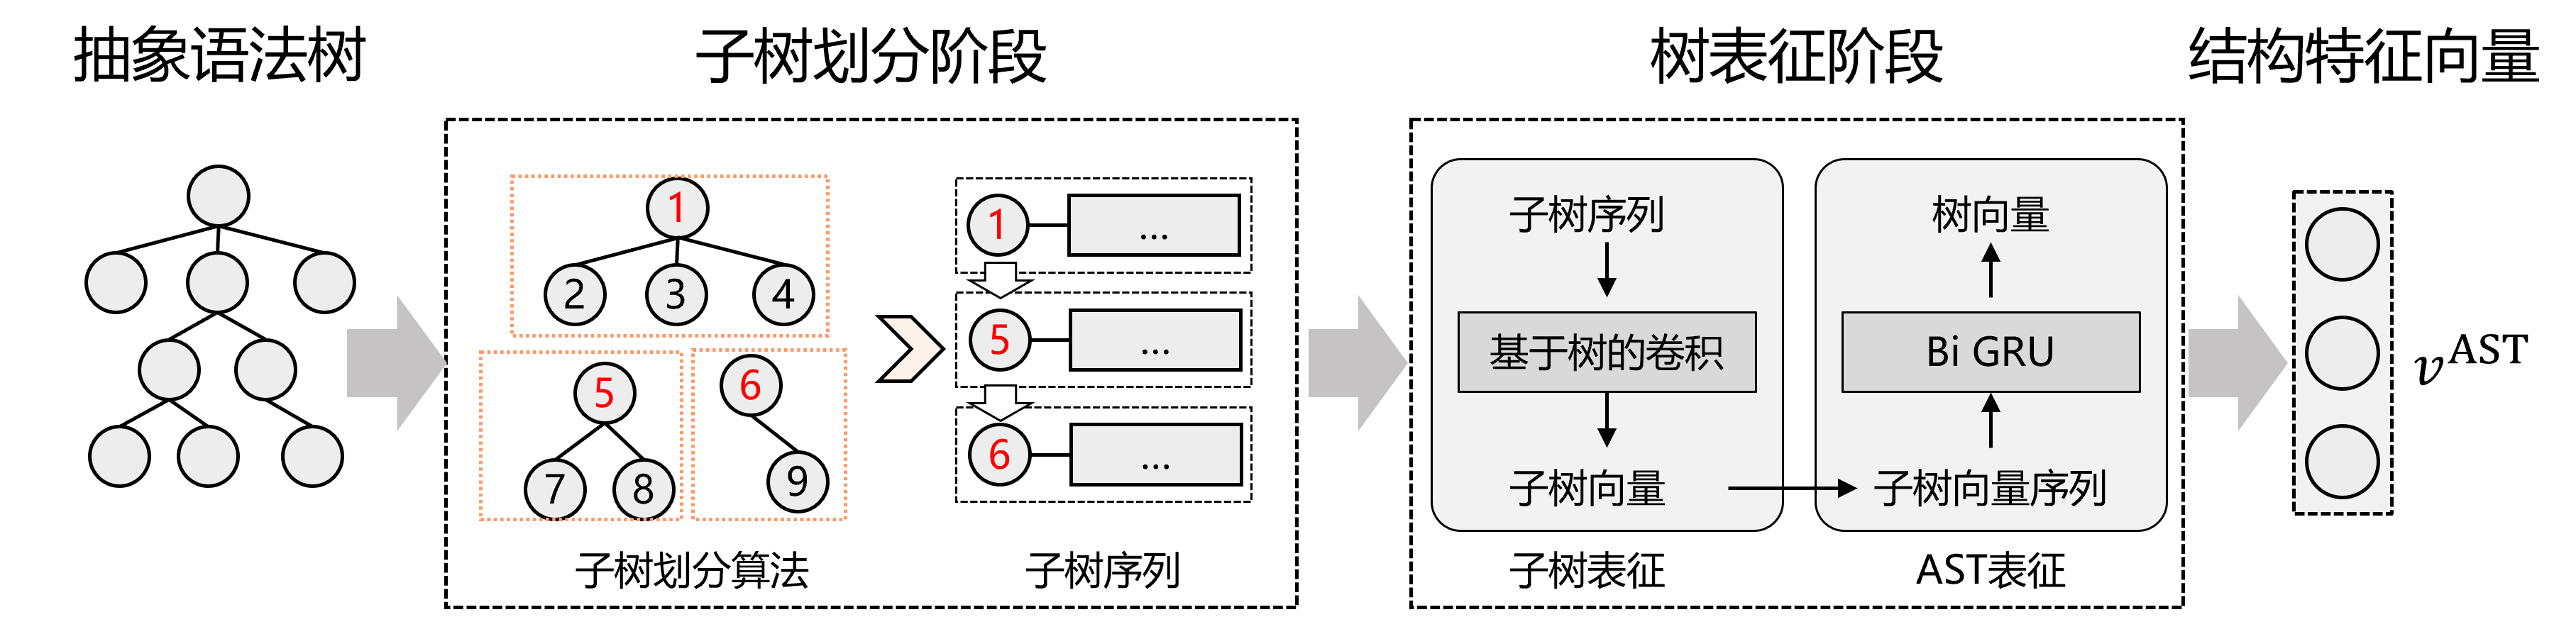
\includegraphics[width=0.95\textwidth]{figures/astframework.png}
  \caption{基于子树划分的抽象语法树表征学习框架}\label{fig:astframework}
\end{figure}

首先,子树划分阶段以代码片段对应的抽象语法树作为训练数据,以抽象语法树的声明节点和语句节点作为切割粒度,设计一个基于先序遍历的子树划分算法,将抽象语法树切分成若干子树,得到对应的子树序列。

其次,树表征阶段以子树序列作为输入,输出代码片段对应的结构特征向量。该阶段分为两个部分,首先针对每一个子树,构建一个基于树的卷积神经网络将子树编码成向量,实现对细粒度语义的捕捉;其次,构建一个基于双向门控循环单元(BiGRU)的神经网络模型,通过最大池化层对子树特征进行压缩,输出一个固定长度的密集向量用来表示代码的结构特征。需要注意的是,在树表征阶段,本文使用两种神经网络模型,前者在语句粒度上对代码信息进行特征提取,后者引入在GRU模型的基础上引入双向结构,从而更好地捕捉序列数据的双向依赖关系。

在上述框架中,本文的创新点主要体现在子树划分阶段的子树划分算法、树表征阶段的树卷积、BiGRU模型设计两方面,下面将围绕这两个创新点来阐述本文的方法。

\subsection{子树划分设计}
\label{subsec:ASTPreModel}

抽象语法树是源代码语法结构的一种抽象表现形式,以树的形式包含了源代码中的语法信息和语法结构,不同的节点类型代表了源代码中的不同元素。其中,声明节点和语句节点是两种关键的节点类型。

声明节点用来定义代码中变量、函数、类等元素的声明,不仅包含了声明的标识符名称,还包含了该标识符的类型信息、作用域以及可能的初始值等。例如,在编译时,编译器可以通过检查声明节点来确保变量在使用前已经被正确声明,并且其类型与使用场景相匹配。

语句节点则用来定义代码的执行语句,如赋值语句、条件语句、循环语句、函数调用等。在AST中,语句节点通常包含了语句的类型、操作数以及可能的控制流信息。例如,在编译条件语句时,编译器可以通过分析语句节点来确定条件表达式的求值结果,并据此决定程序的执行路径。

抽象语法树存在因为树规模过大、高度过深导致的梯度消失问题,本文设计了一个基于先序遍历的子树划分算法,通过在语句粒度上对AST进行划分,在减少树高度的同时,实现对细粒度语义的捕捉。下面首先对本文提出的子树划分算法涉及到的基本元素进行定义,接着详细介绍整个算法流程。

\textbf{定义4.1.}抽象语法树语句节点集合:对于一个代码片段的AST,假设该AST的节点集合为$T = \left\{T_1,T_2,\ldots,T_n\right\}$,影响子树划分标准的语句节点包括:块语句、FOR循环语句、While循环语句、条件语句、返回语句,因此本文定义这些不同类型语句节点构成集合$S = \left\{BlockStatement,IfStatement,WhileStatement,ForStatement,\notag \right.\\\left.ReturnStatement\right\}$。

具体来说,子树划分算法需要寻找一个子树节点集合,表示为$SubT = \left\{SubT_i |\notag \right.\\\left. SubT \in T, SubT \in S,i=1,2,\ldots,k\left(k<n\right)\right\}$,其中集合$SubT$通过先序遍历AST节点获得,$n$表示AST中节点的总数量。

子树划分$split\_AST$算法的伪代码如\ref{alg2}所示,该算法有两个输入:根节点$Root\_Node$、语句节点集合$S$,输出为子树序列$SubTrees$。该算法的目的是按照先序遍历抽象语法树,根据给定的语句节点集合$S$,从根节点$Root\_Node$开始,判断每个子节点$child\_node$,是否需要将其作为新的子树进行切分(算法第4行),如果子节点属于语句节点集合,则直接加入子树节点集合中(算法第5行),否则需要继续遍历,找到包含子节点的子树,进行递归切分(算法第11行),最终得到子树节点列表,即子树序列$SubTrees$。

\begin{algorithm}[ht]  
	\renewcommand{\algorithmicrequire}{\textbf{Input:}}
	\renewcommand{\algorithmicensure}{\textbf{Output:}}
	\caption{Subtree partitioning algorithm $\left(split\_AST\right)$}  
	\label{alg2}
	\begin{algorithmic}[1]
    \Require Root node of abstract syntax tree:$Root\_Node$
    \Require Node set:$S$
		\Ensure SubTree set:$SubTrees$
    \State $SubTrees = \left\{\right\} $    
    \State SubTrees.append$\left(Root\_Node\right)$
		\For{child\_node $in$ Root\_Node.children}
      \If {child\_node $\in$ S} \Comment{判断是否是语句节点}
        \State SubTrees.append$\left(child\_node\right)$
      \Else
        \For{subtree $in$ SubTrees} \Comment{继续遍历子树}
          \If {child\_node $\in$ SubTrees.descendant}
            \State SubTrees.append$\left(child\_node\right)$
          \Else
            \State $ split\_AST\left(subtree\right)$ \Comment{递归切分}
          \EndIf
        \EndFor
      \EndIf
    \EndFor \\
    \Return $SubTrees$
	\end{algorithmic}
\end{algorithm}

具体地,如图\ref{fig:astshili}所示,(a)为示例代码片段,(b)为利用代码分析工具Joern生成得到抽象语法树T,(c)为利用子树划分算法将其切分为一系列子树SubT。其中,以Method为根节点,其名称为main,body节点则代表了内部代码块,该块中包含三棵变量声明子树(Local)、一棵FOR循环条件子树(ForStatement)、一棵函数声明子树(Function)以及返回语句子树(ReturnStatement),而FOR循环条件子树内部包含一课If条件句法子树(IfStatement)。

\begin{figure}[H]
  \centering
  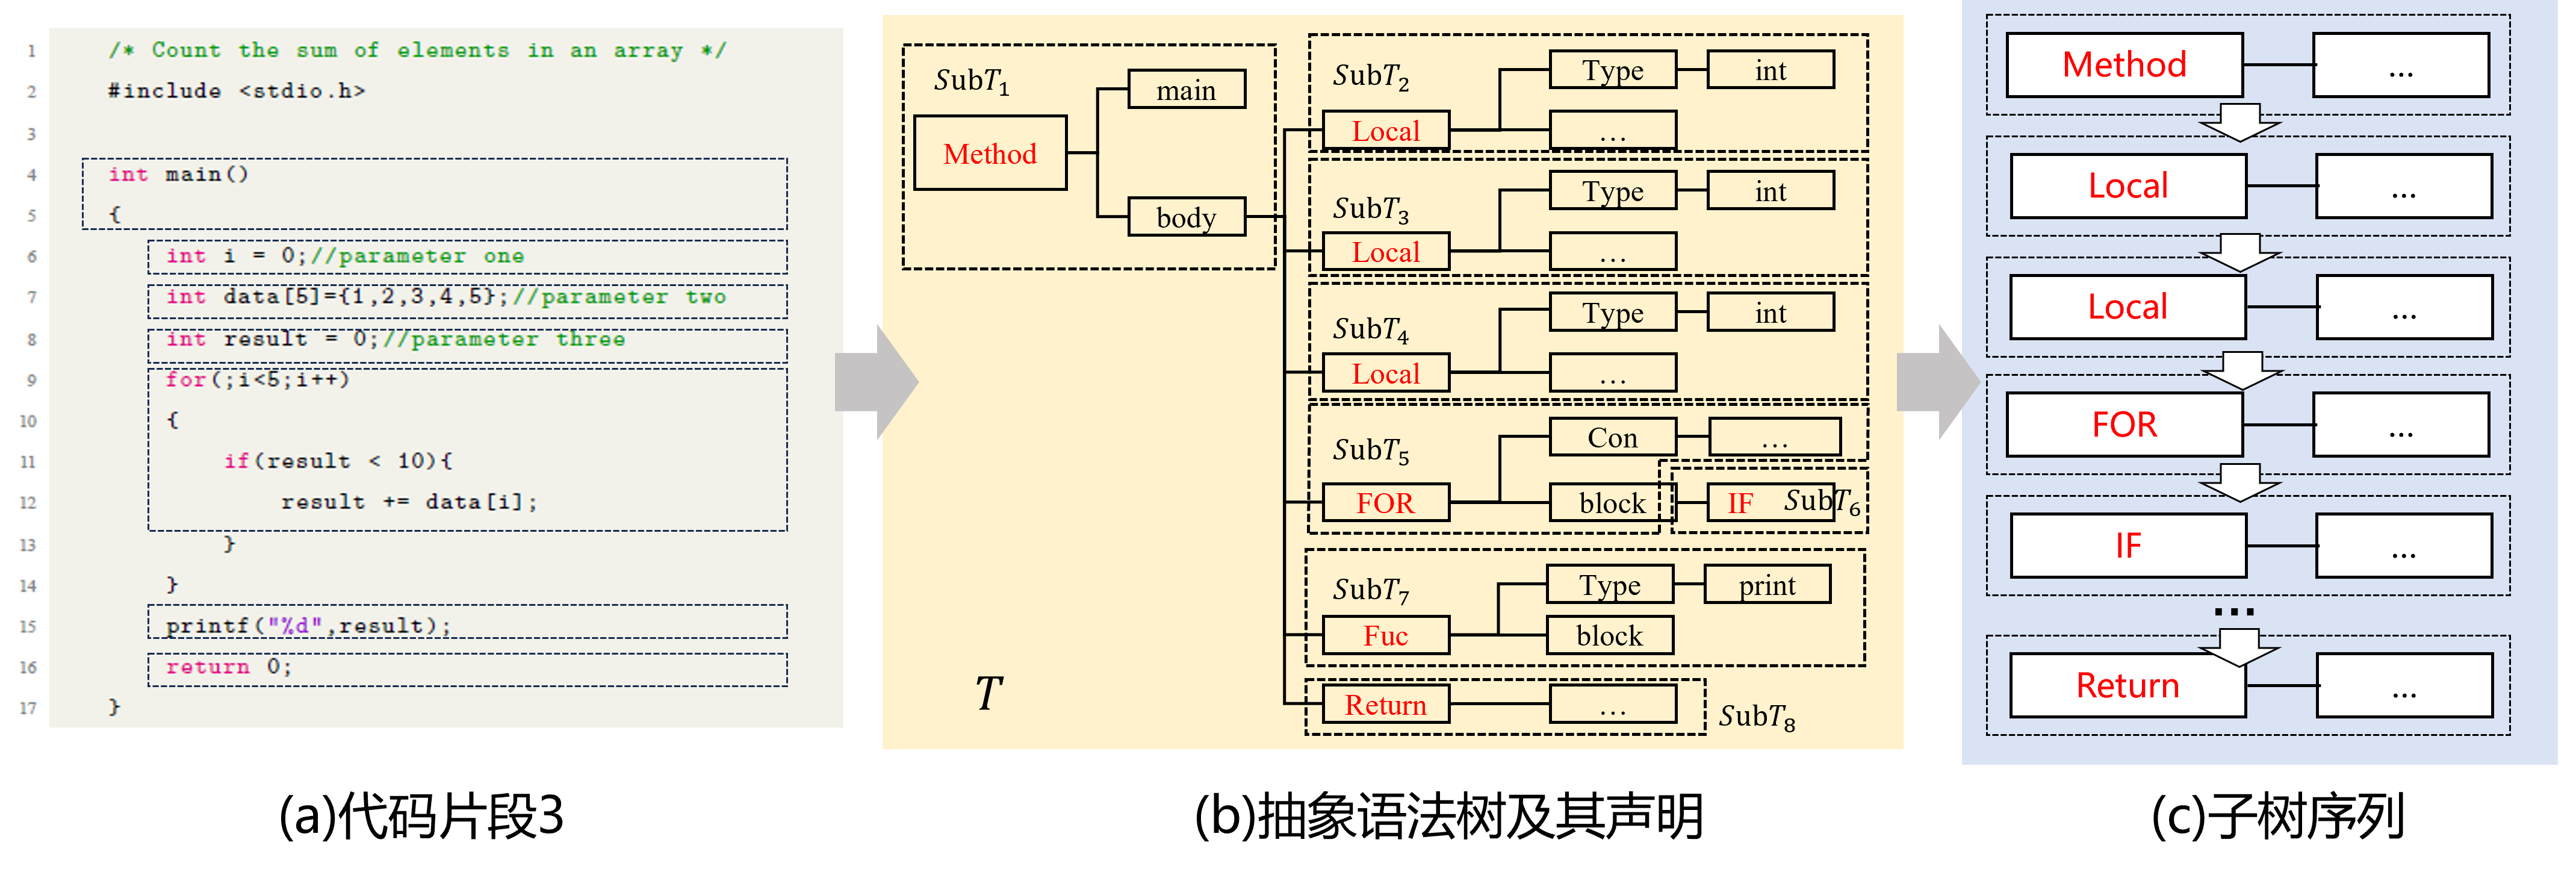
\includegraphics[width=0.95\textwidth]{figures/astshili.png}
  \caption{子树划分算法示例}\label{fig:astshili}
\end{figure}

% \lstset{language=C}
% \begin{lstlisting}
%     /* Count the sum of elements in an array */
%     #include <stdio.h>
    
%     int main()
%     {
%         int i = 0;//parameter one
%         int data[5]={1,2,3,4,5};//parameter two
%         int result = 0;//parameter three
%         for(;i<5;i++)
%         {
%             if(result < 10){
%                 result += data[i];
%             }
%         }
%         printf("%d",result); 
%         return 0;
%     }
% \end{lstlisting}

\subsection{抽象语法树表征学习设计}
\label{subsec:ASTModel}
(1)结构设计

为了提高抽象语法树维度代码表征能力,本文选取树卷积网络对上述得到子树序列进行建模,使用双向门控循环单元(BiGRU)对整个树进行建模。具体的模型设计如图\ref{fig:astmodel}所示。该模型主要包括输入层、子树卷积层、双向门控循环层(BiGRU)、最大池化层、输出层。
\begin{figure}[H]
  \centering
  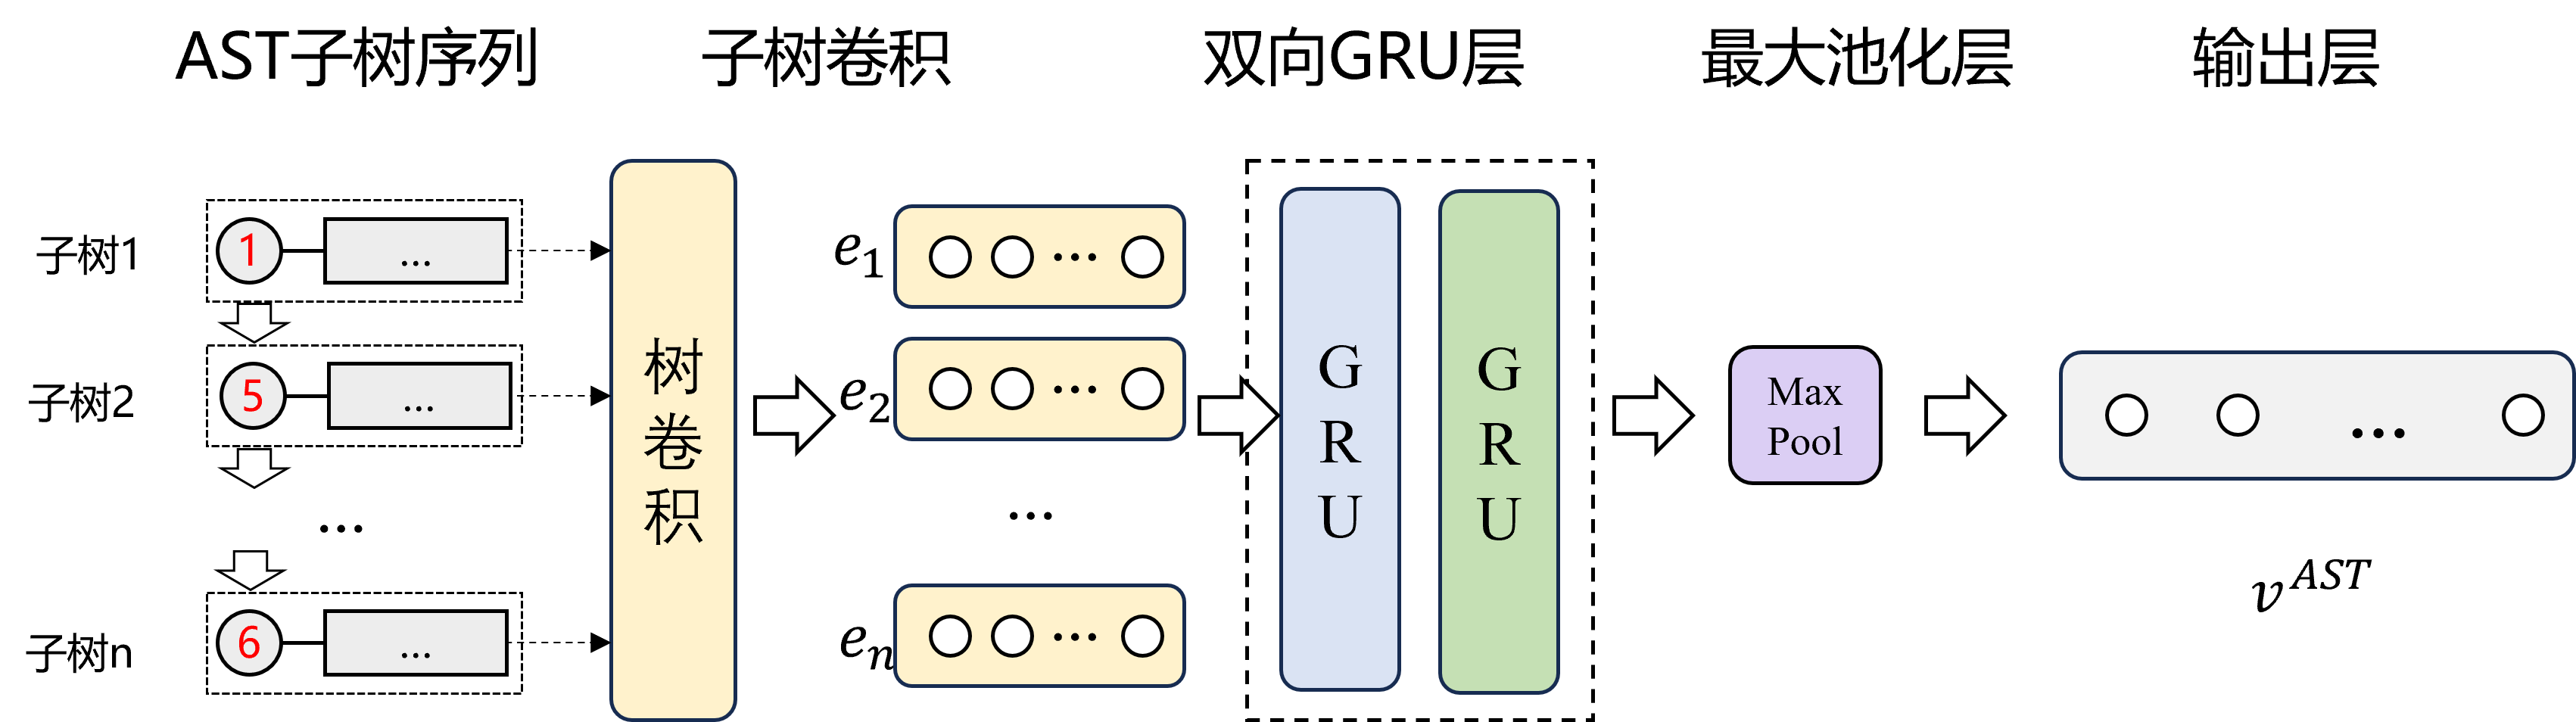
\includegraphics[width=0.85\textwidth]{figures/astmodel.png}
  \caption{抽象语法树维度代码表征模型结构}\label{fig:astmodel}
\end{figure}

\ding{172}输入层:输入层用于向模型输入训练数据,在本方法中模型的输入为经过子树划分得到的子树序列。\ding{173}子树卷积层:针对子树序列中的每一个子树,通过基于树的卷积,捕获语句粒度语义信息。\ding{174}双向门控循环层:由两层GRU构成,同时捕获序列的双向语义信息。\ding{175}最大池化层:总结子树序列的输入特征,并将其缩减为一个单一的密集向量。\ding{176}输出层:每个抽象语法树对应一个输出。

(2) 模型选型

树表征阶段包含两个步骤:子树表征、整树表征。因此本文设计了两个神经网络模型:前者的输入是子树序列,针对每个子树进行基于树的卷积,在子树粒度上对代码进行信息提取;后者的输入是子树向量序列,针对所有子树的特征进行双向特征提取,并整合整棵树的信息,得到一个结构特征向量。

(2.1)子树表征模型

卷积神经网络(Convolutional Neural Network,CNN)是一种深度学习模型,其架构包括多个卷积层、池化层和全连接层。其中,卷积层负责从输入数据中提取特征,池化层用于降低数据维度,全连接层则用于将前面各层的特征映射到输出空间。其中,卷积思想是指将一个固定大小的窗口(通常被称为卷积核)在输入数据上按照一定的步长进行滑动,并对每个窗口中的局部片段进行特征提取,最后得到一系列特征,每个特征对应一个卷积核提取的特征。它能够将输入数据从底层到高层逐步抽象化,形成层次化的特征表示。

常见的卷积核通常都是正方形的,但树形结构通常是不规则,因此有研究\cite{8813290}提出了基于树的卷积神经网络。该网络的核心思想是将卷积操作扩展到树形结构上。通过定义在树上的卷积核,可以捕获树的节点与其邻居之间的局部特征。这种局部感知的方式与传统的卷积神经网络类似,但不同的是,其卷积核是三角形的,能够在不规则的树形结构上进行。基于树的卷积如下图\ref{fig:TreeBaseConvolution}所示。

\begin{figure}[H]
  \centering
  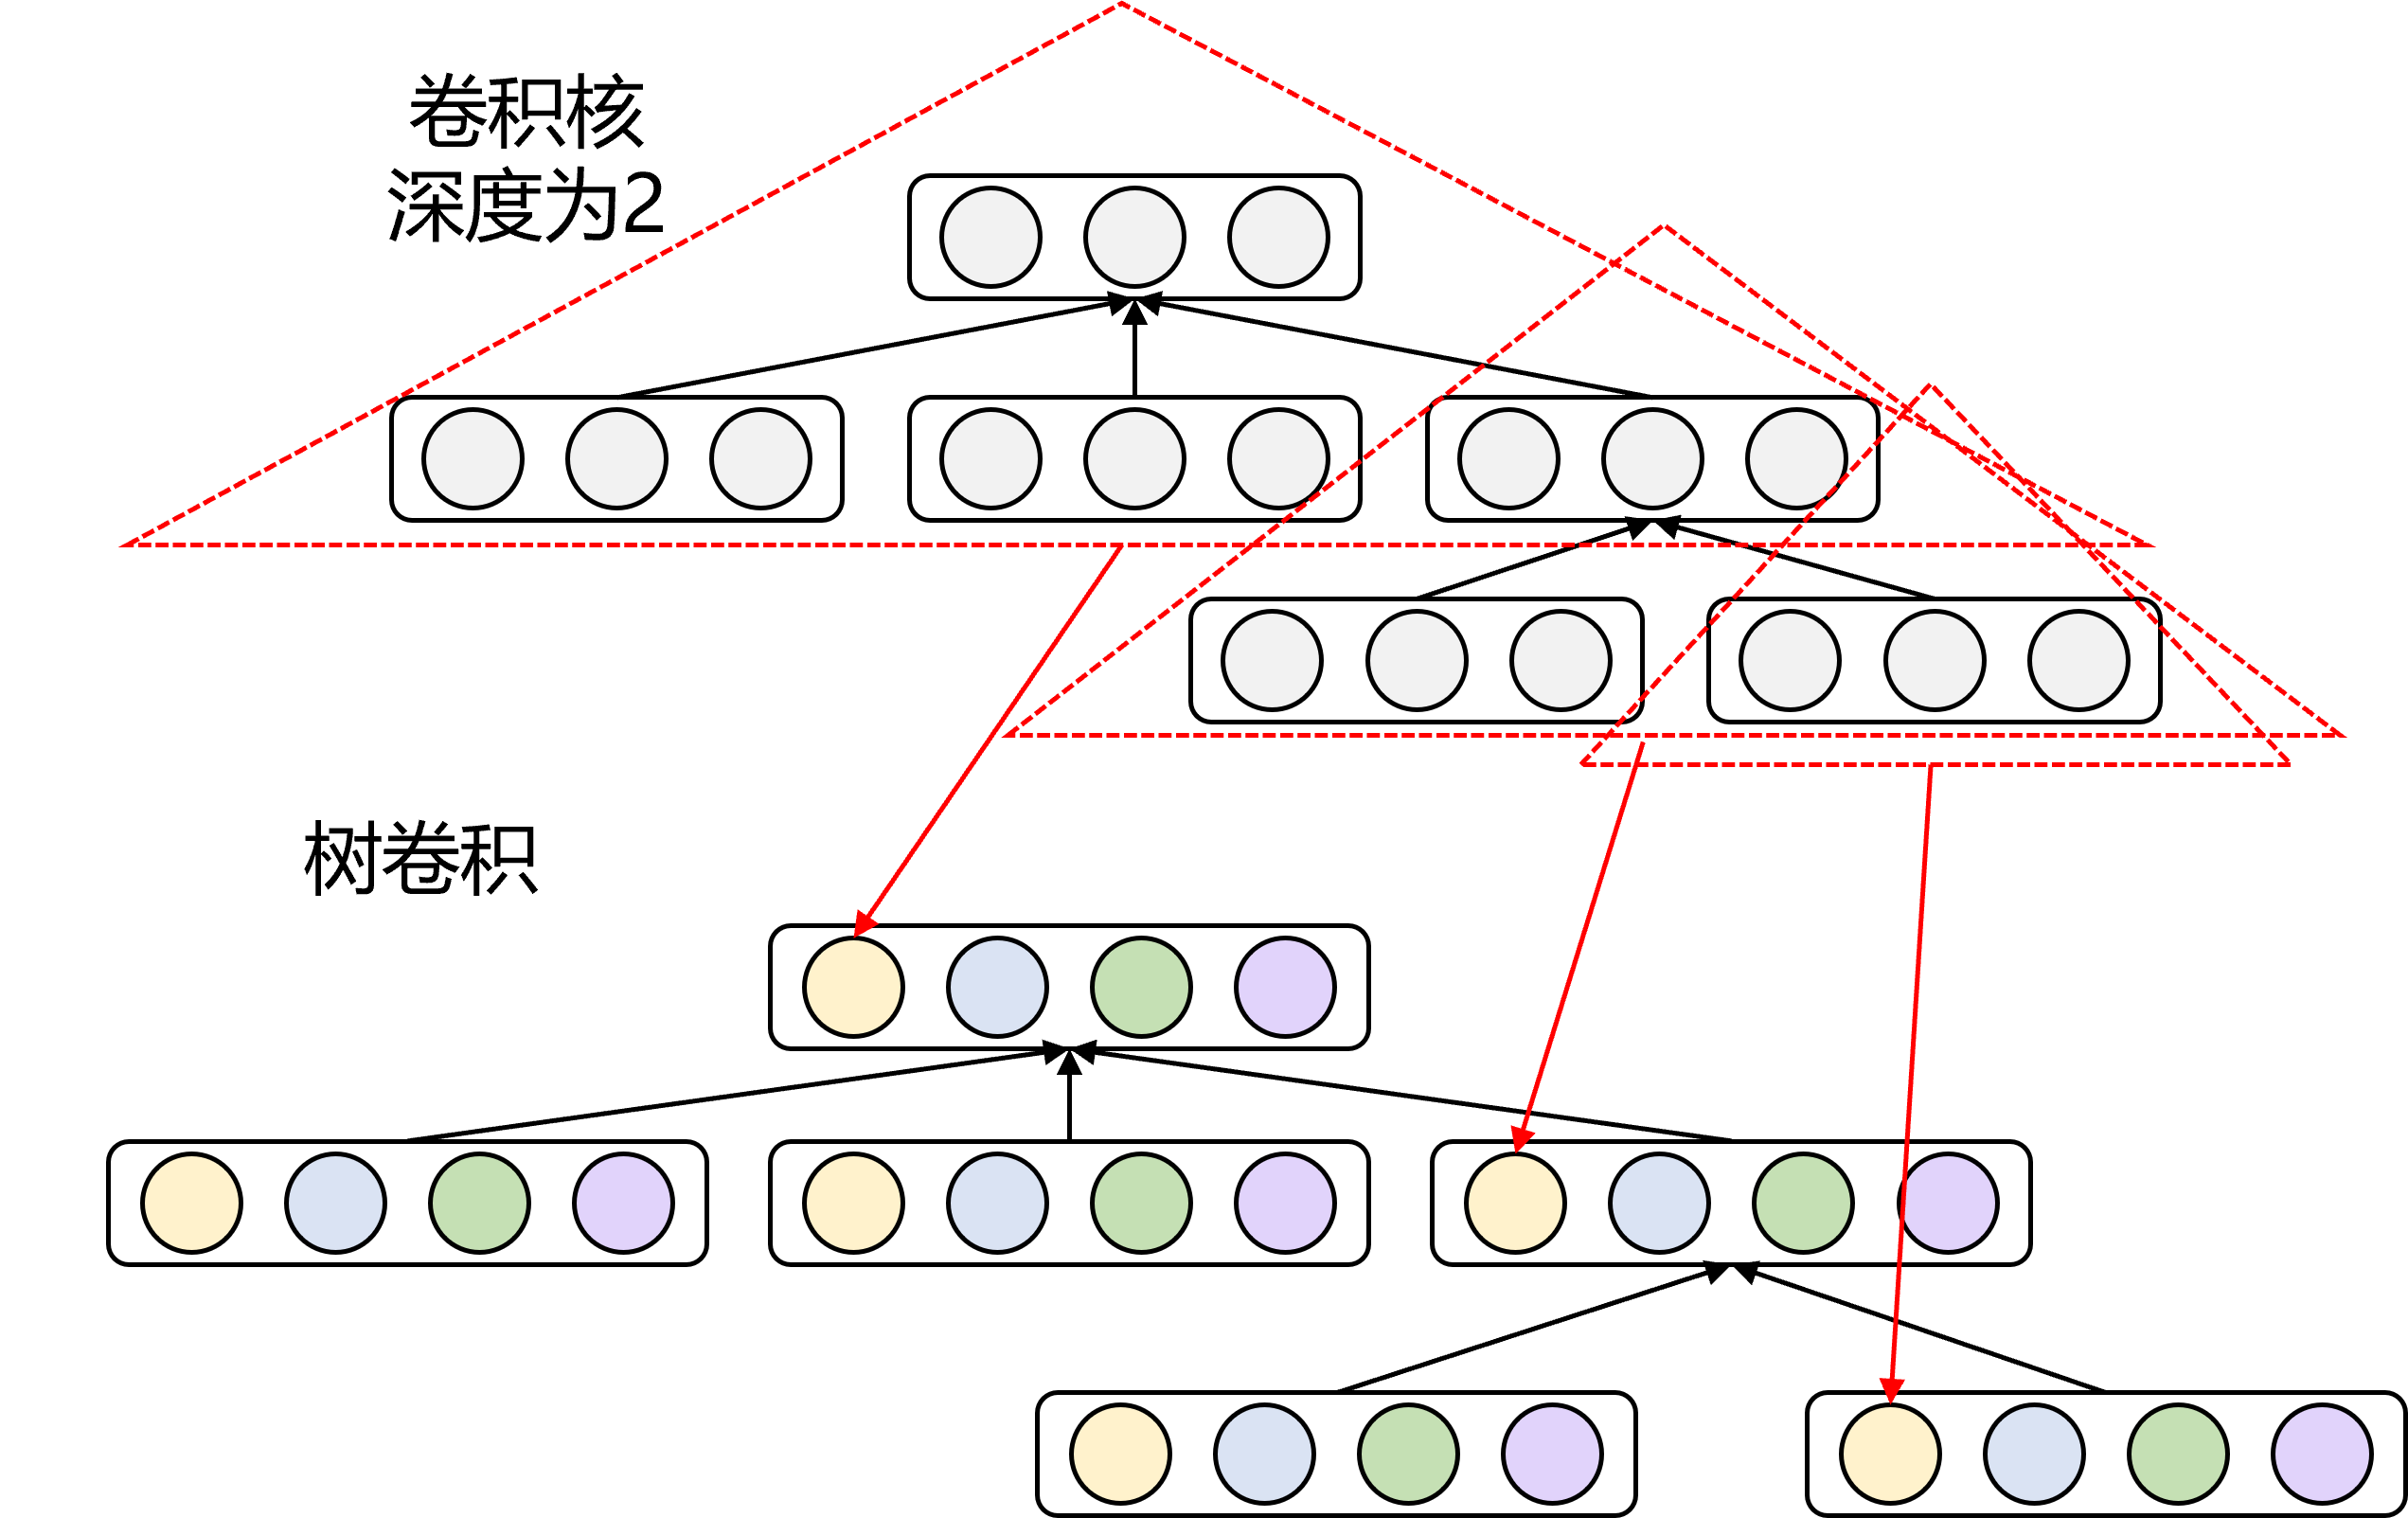
\includegraphics[width=0.65\textwidth]{figures/TreeBaseConvolution.png}
  \caption{基于树的卷积神经网络模型结构}\label{fig:TreeBaseConvolution}
\end{figure}

在基于树的卷积神经网络中,每个节点都与其邻居节点相连,形成一个局部邻域。卷积核在这个局部邻域上进行滑动,计算节点与其邻居的加权和,从而提取出特征。用数学公式表示,卷积核的滑动尺寸是$d$,它表示每个滑动窗口能够包括的树的层数。在这个窗口内包含$n$个节点$\left(x_1,x_2,\ldots,x_n\right)$,其中,$x_i \in \mathbb{R}^{N_{f}}$,$N_{f}$表示每个节点建模后的向量大小。使用公式\ref{e4.1}可以对滑动窗口内$n$个节点进行卷积得到基于树的卷积神经网络输出。
\begin{equation}\label{e4.1}
  \begin{split}
    y = \tanh \left(\sum_{i=1}^{n} W_{\text{conv}, i} \cdot x_{i}+b_{\text{conv}}\right)
  \end{split}
\end{equation}

其中,$y, b_{\text{conv}} \in \mathbb{R}^{N_{f}}, W_{\text{conv}, i} \in \mathbb{R}^{N_{c} \times N_{f}}$,$N_{c}$为最后卷积得到的向量长度。具体地,在上图\ref{fig:TreeBaseConvolution}的例子中,红色三角形表示卷积核,固定深度$d$为2,最后输出的卷积向量长度$N_{c}$为4。树结构在卷积前后保持相同的形状,而每个节点向量的维数由原来的3维变为4维。

基于树的卷积网络模型存在一个限制:其子节点的数量被限制为两个。但实际上,AST理论上可以存在无限数量的子节点,每次滑动窗口中的节点数$n$难以固定,从而导致无法确定权重矩阵的数量,即公式\ref{e4.9}中的$W_{conv,i}$。现有研究的解决方法是预先定义一组规则将抽象语法树转化为二叉树,然后再进行树卷积。这种处理方式,会改变源代码原有的语义,从而难以捕捉远程依赖关系,甚至丢失一些上下文信息,因此本文采用研究\cite{8813290}中提出的连续二叉树概念,将AST的每一个子树都看作二叉树,而不管它的形状和尺寸。图\ref{fig:Continuous}展示了连续二叉树的定义。

\begin{figure}[H]
  \centering
  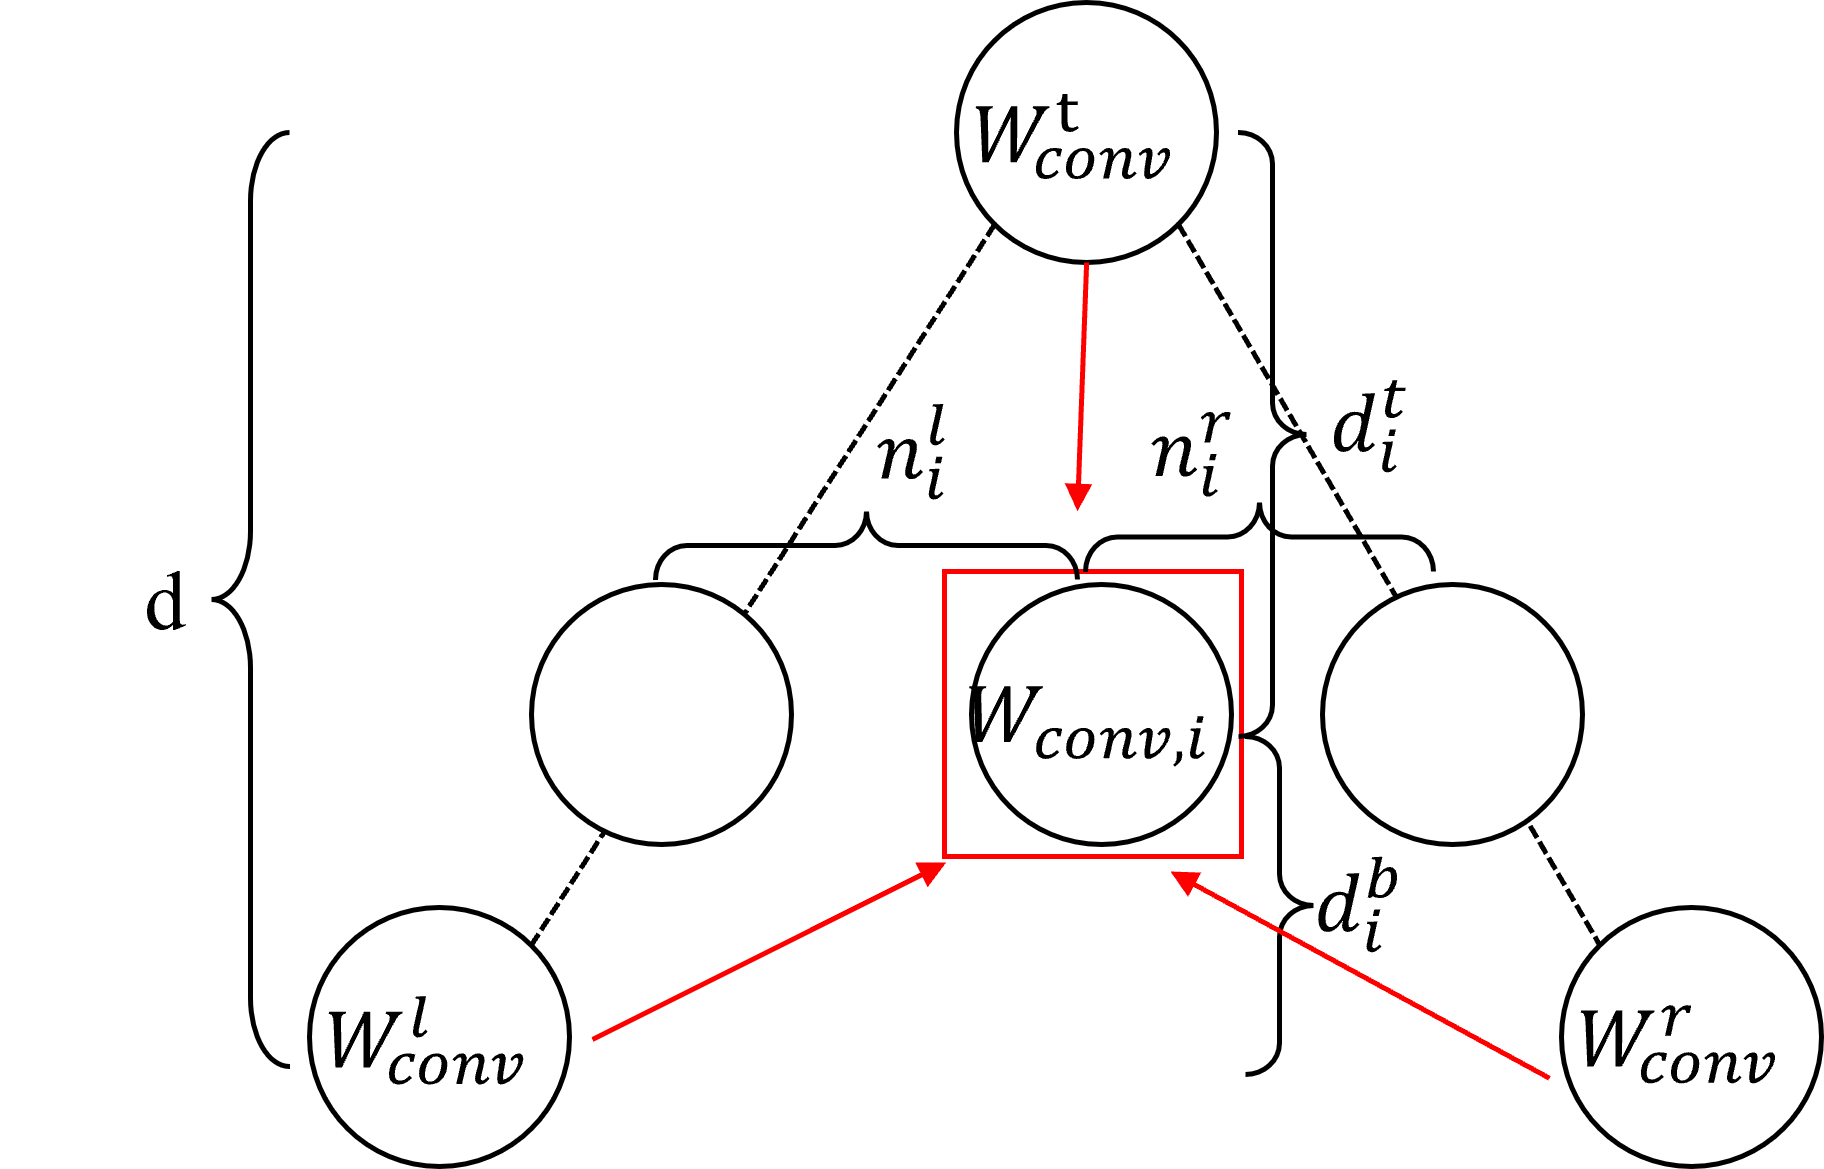
\includegraphics[width=0.6\textwidth]{figures/Continuous Binary Tree.png}
  \caption{连续二叉树}\label{fig:Continuous}
\end{figure}

具体地,针对滑动窗口中的节点,需要设置三个变量:$W_{\text{conv}}^{t},W_{\text{conv}}^{l},W_{\text{conv}}^{r}$分别代表当前节点距离树形上、左、右三个方向,其卷积矩阵$W_{conv,i}$是这三个变量的线性组合,其系数根据节点在当前滑动窗口中的相对位置计算,具体公式为\ref{e4.2}:
\begin{equation}\label{e4.2}
  \begin{split}
    W_{\text{conv}, i}=\frac{d_{i}^{b}}{d_{i}^{b}+d_{i}^{t}} W_{\text{conv}}^{t}+\frac{d_{i}^{t}}{d_{i}^{b}+d_{i}^{t}} W_{\text{conv}, i}^{b}
  \end{split}
\end{equation}

其中,$d_{i}^{t}$表示当前节点距离树形顶点的距离,$d_{i}^{b}$表示当前节点距离树形左右顶点构成的边的距离,两者相加为$d$,即$d_{i}^{t} + d_{i}^{b} = d$。上式中$W_{\text{conv}, i}^{b}$有如下定义:

\begin{equation}\label{e4.3}
  \begin{split}
    \begin{array}{l}
      W_{\text{conv}, i}^{b}= 
      \left\{\begin{array}{ll}
      \frac{n_{i}^{r}}{n_{i}^{r}+n_{i}^{l}} W_{\text {conv}}^{l}+\frac{n_{i}^{l}}{n_{i}^{r}+n_{i}^{l}} W_{\text{conv}}^{r} & n_{i}^{l} \geq 1 \text { or } n_{i}^{r} \geq 1, \\
      \frac{1}{2} W_{\text{con}}^{l}+\frac{1}{2} W_{\text{conv}}^{r} & n_{i}^{l}=n_{i}^{r}=0 .
      \end{array}\right.
      \end{array}
  \end{split}
\end{equation}

其中,$n$表示树的同一层左右两个方向的兄弟节点个数。通过上述公式,可以计算在一个三角形的卷积窗口中,当节点越接近顶点,其$W_{\text{conv}}^{t}$的权重值越大,当节点越接近树形结构左下节点,其$W_{\text{conv}}^{l}$的权重值越大,当节点越接近树形节点结构右下节点,其$W_{\text{conv}}^{r}$的权重值越大。在具体实验中,本文设置滑动窗口的$d$值为2。

(2.2)整树表征模型

\ref{subsec:TokenModel}小节中提到长短期记忆网络LSTM模型针对长依赖问题效果明显,解决了传统RNN模型中存在的梯度消失问题,但是LSTM模型同样存在缺陷,其LSTM单元内包含三个门,机制相对复杂,计算成本会有所提高,因此,有研究提出了门控循环单元GRU,将遗忘门和输入门进行组装,形成一个新的更新门,这种改进使得GRU在模型参数和计算效率上通常优于LSTM。GRU单元的时序结构如下如\ref{fig:GRU}所示,每个GRU单元都包含两个门:重置门(Reset Gate)和更新门(Update Gate),通过重置门和更新门来直接控制信息的流动和隐藏状态的信息更新。

\begin{figure}[H]
  \centering
  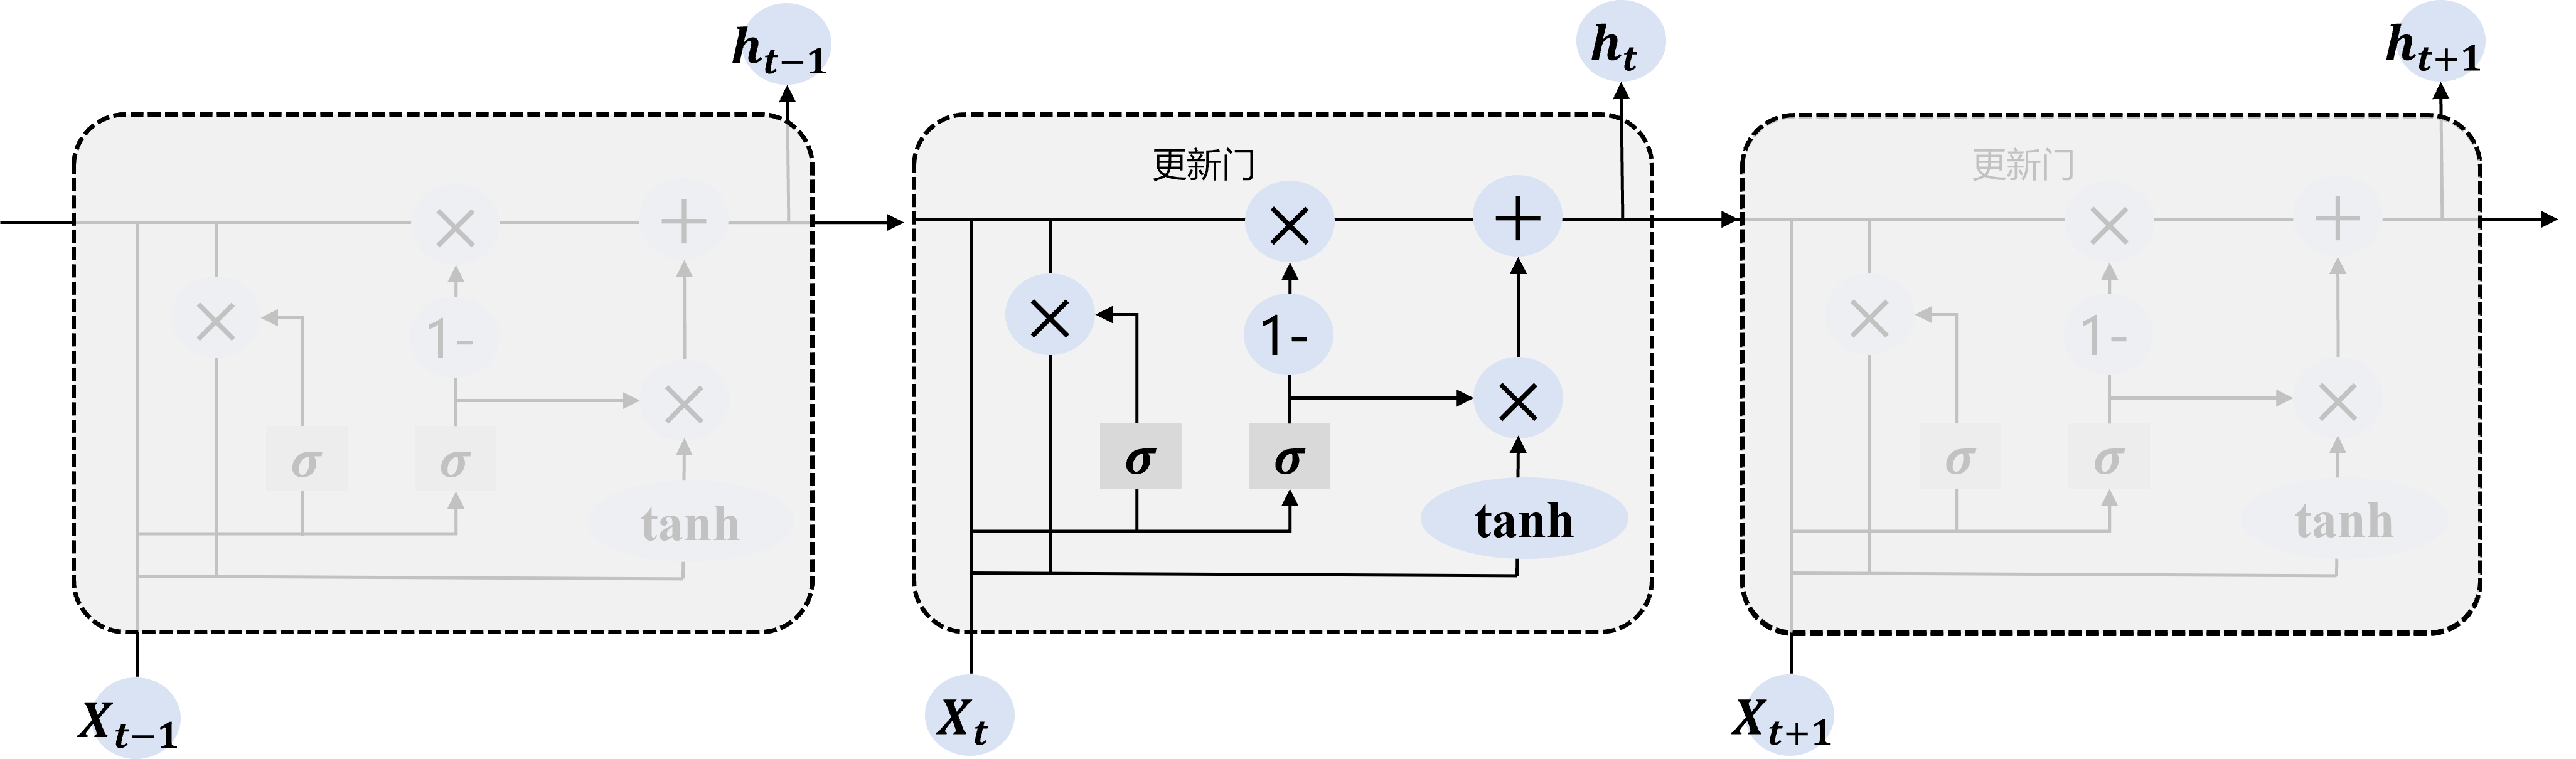
\includegraphics[width=0.85\textwidth]{figures/GRU.png}
  \caption{GRU模型时序结构图}\label{fig:GRU}
\end{figure}

具体来说,首先会根据当前时间步的输入$x_{t}$和上一时间步的隐藏状态$h_{t-1}$计算出重置门和更新门的值,具体的计算公式见\ref{e4.4}。
\begin{equation}\label{e4.4}
  \begin{split}
    z_{t} = \sigma \left(W_{u} \cdot \left[h_{t-1},x_{t}\right] + b_z \right)
    \\
    r_{t} = \sigma \left(W_{r} \cdot \left[h_{t-1},x_{t}\right]  + b_r \right)
  \end{split}
\end{equation}

然后,输入重置门,对上一个时间步的隐藏状态进行处理,得到一个新的候选隐藏状态$\widetilde{h_t}$。其中,重置门用来控制上一个时间步的信息有多少应该被遗忘。具体地,通过公式\ref{e4.5}计算一个介于-1到1之间的值,决定上一个时间步的隐藏状态有多少信息应该被保留或遗忘,得出的值越接近0越有可能被丢弃,越接近1越有可能被记住。
\begin{equation}\label{e4.5}
  \begin{split}
    \widetilde{h_t} &= \tanh \left(W_x \cdot x_t \otimes U_h \cdot\left(r_t \cdot h_{t-1}\right) + b_h  \right)
  \end{split}
\end{equation}

接着,输入更新门,将新的候选隐藏状态$\widetilde{h_t}$和上一个时间步的隐藏状态$h_{t-1}$进行加权组合,得到当前时刻的隐藏状态$h_t$,如公式\ref{e4.6}所示。其中,更新门用来控制新输入的信息和上一个时间步的信息应该如何结合。具体地,通过公式\ref{e4.7} 决定当前时刻的隐藏状态应该有多少信息来自上一时刻的隐藏状态,以及有多少信息来自当前时刻的输入和重置门处理后的结果。通过更新门,GRU能够平衡新旧信息的影响,从而有效地捕捉序列数据中的长期依赖关系。最后,当前时刻的隐藏状态会被输出。

\begin{equation}\label{e4.6}
  \begin{split}
   h_t &= \left(1- z_t\right) \otimes h_{t-1} +  z_t \otimes \widetilde{h_t}
  \end{split}
\end{equation}

同样地,在抽象语法树中,某一个节点的状态不仅和前面层的节点状态有关,也可能和后一层的节点状态有关。为了更好地提高模型对AST子序列的表征能力,本文选择了双向BiGRU模型来进行树代码表征,模型的结构如下图\ref{fig:BiGRU}所示。BiGRU模型结构结合了双向RNN(双向循环神经网络)和GRU(门控循环单元)的优点,通过其双向结构能够更有效地学习并保持长期的信息流,从而使得当前时刻的输出与前后时刻的状态都产生联系,在处理长序列数据时表现出色,在具有较快收敛速度、较强学习能力等优点的同时,还能减少梯度消失问题。

\begin{figure}[H]
  \centering
  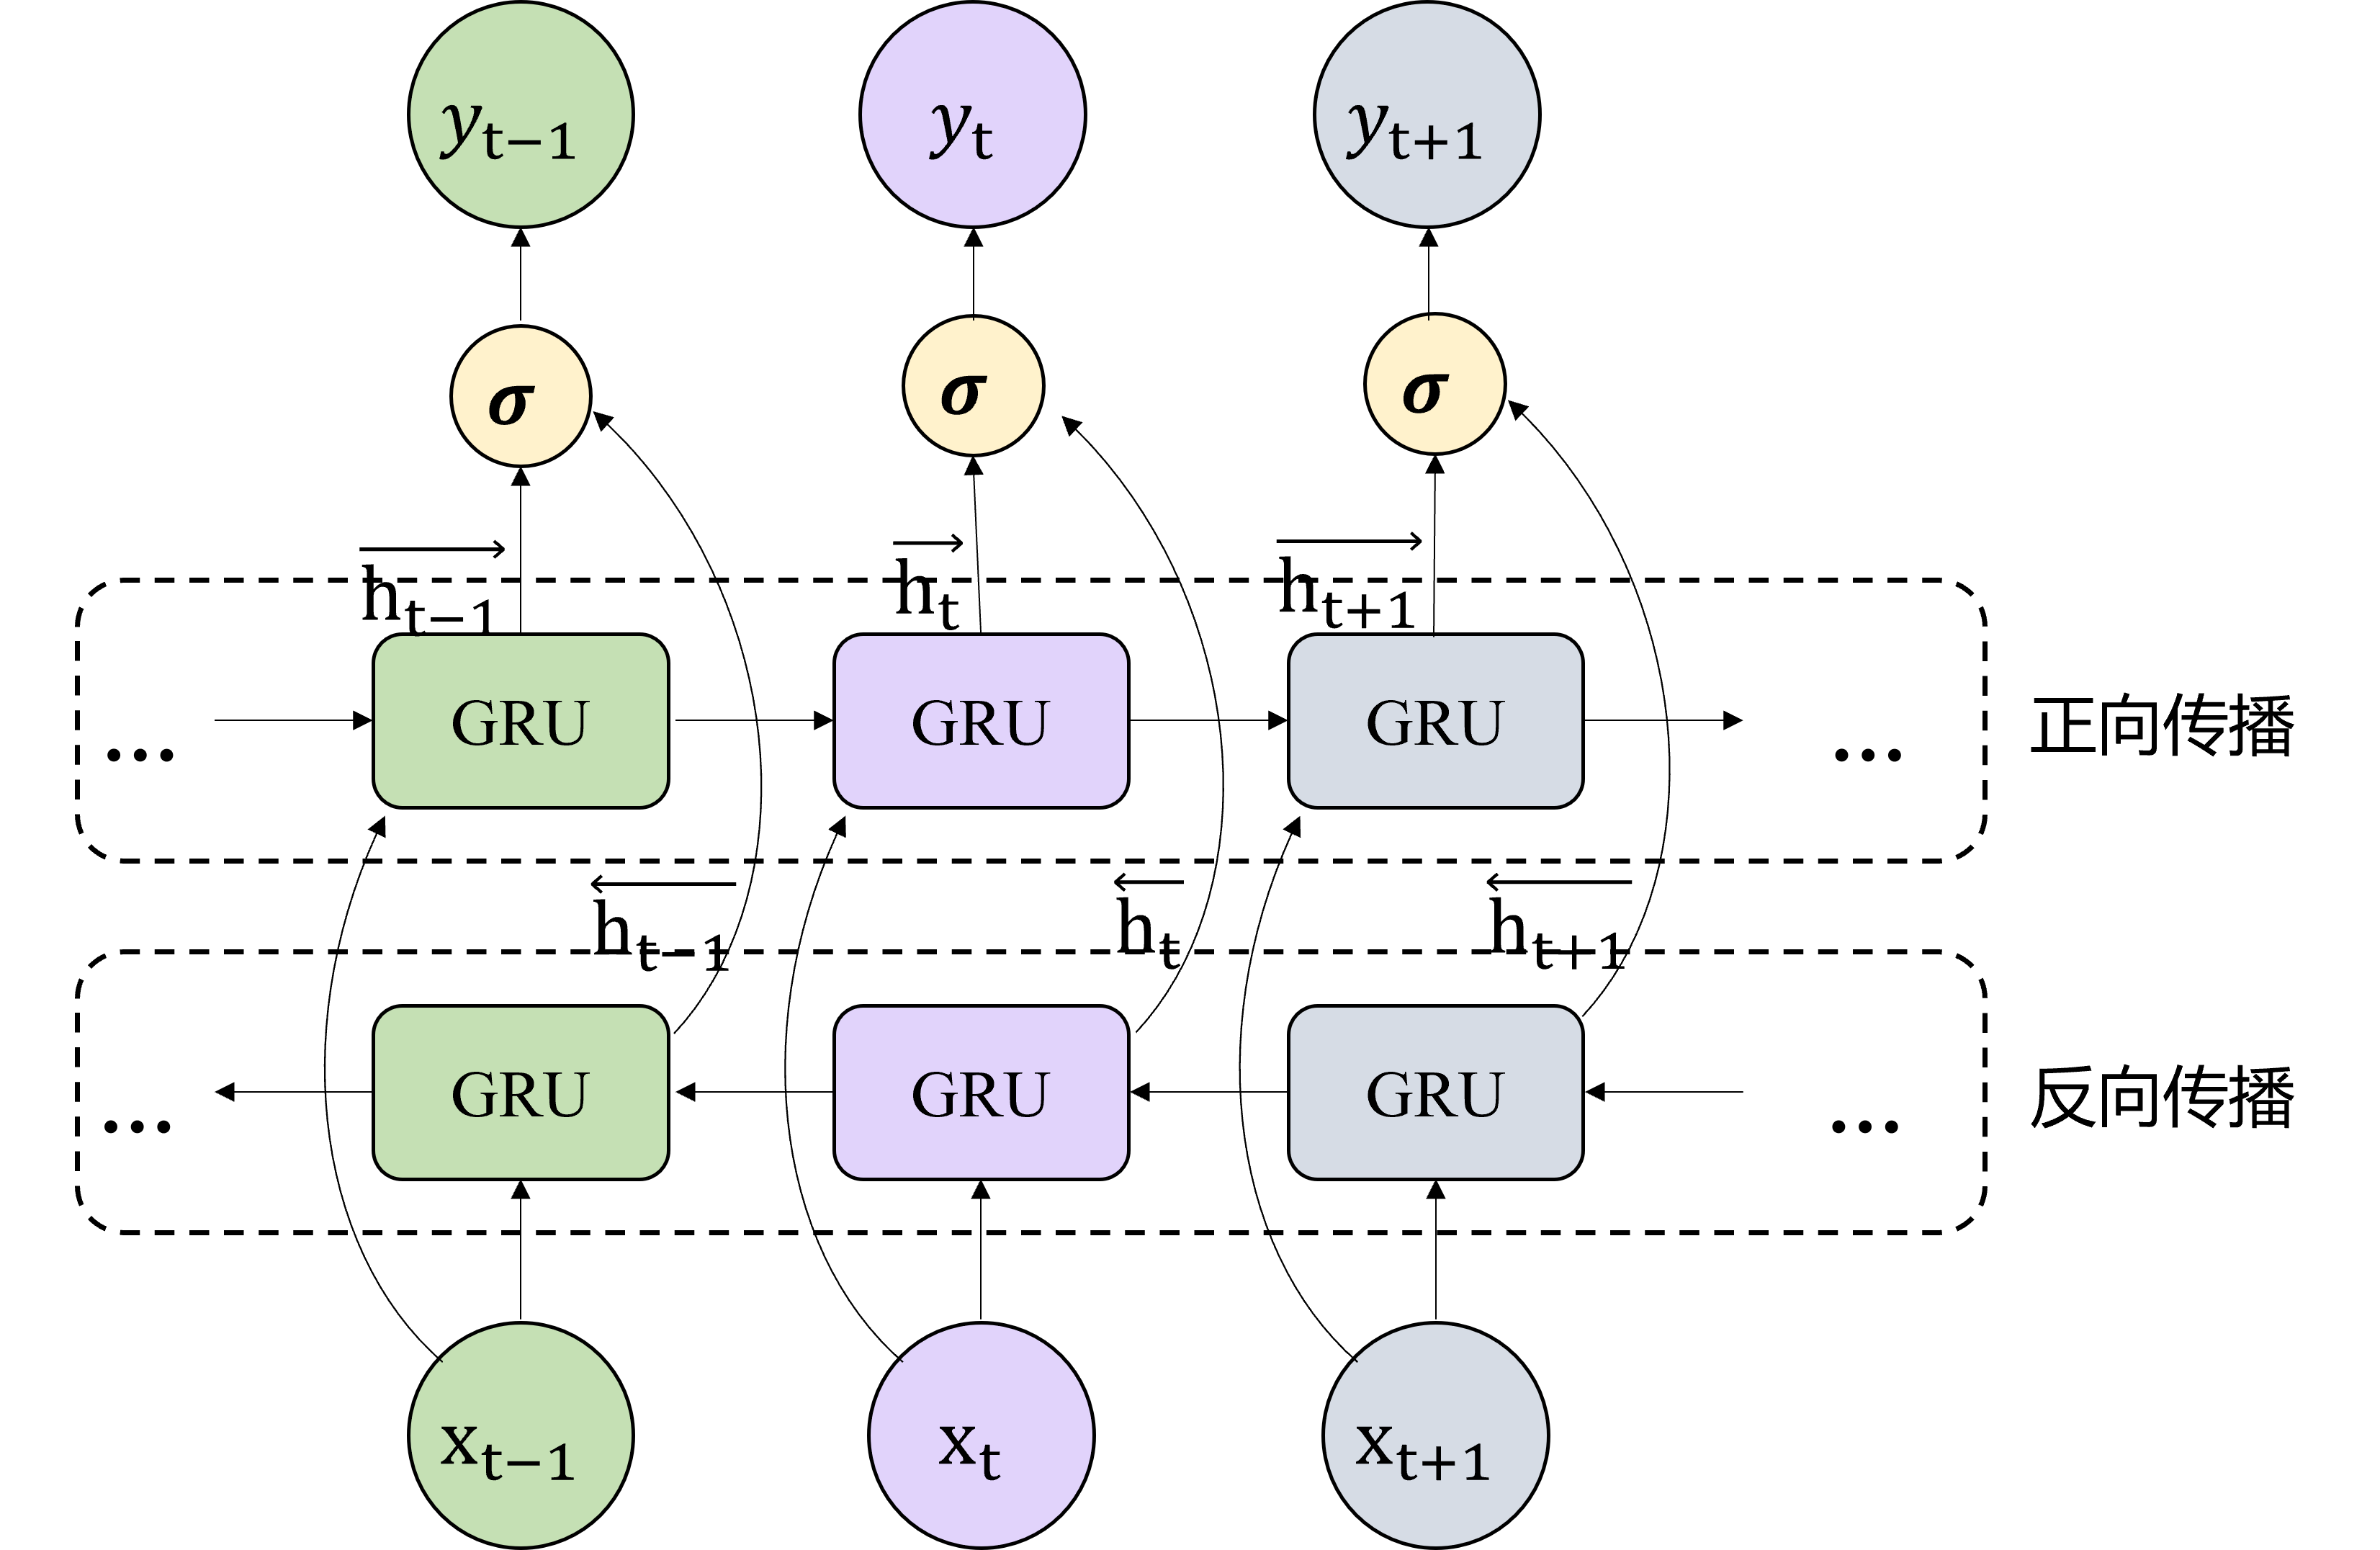
\includegraphics[width=0.5\textwidth]{figures/BiGRU.png}
  \caption{BiGRU模型结构}\label{fig:BiGRU}
\end{figure}

和\ref{subsec:TokenModel}提出的双向长短时记忆模型相比,GRU结构简单,参数简单,因此通常可以更快收敛到最优解,从而节省计算资源和时间。整个模型,除了子单元有所改变外,架构不变。这里不展开介绍,仅给出公式\ref{e4.7}。
\begin{equation}\label{e4.7}
  \begin{split}
    \overrightarrow{y_t} &= W_0 \cdot GRU\left(x_{t},\overrightarrow{h_{t-1}}\right) + b_0
    \\
    \overleftarrow{y_t} &= W_0 \cdot GRU\left(x_{t},\overleftarrow{h_{t-1}}\right) + b_0
    \\
    y_t &= \overrightarrow{y_t} \oplus\overleftarrow{y_t}
  \end{split}
\end{equation}


\section{AST表征方法具体实现}
\label{sec:ASTachieve}
在介绍具体实现之前,本节首先给出AST表征方法的输入:经过\ref{subsec:Preprocess}小节的代码预处理阶段,得到示例代码片段\ref{fig:code}对应的抽象语法树,如图\ref{fig:astcode}所示。仔细分析可以看出代码片段\ref{fig:ast1}对应的抽象语法树在FOR循环内部一共有13个子节点,子树高度为4;代码片段\ref{fig:ast2}对应的抽象语法树在WHILE循环内部也包含13个子节点,子树的高读为4,两者子节点个数相同;而代码片段\ref{fig:ast3}对应的抽象语法树在FOR循环中共有18个子节点,子树高度为6,与代码片段\ref{fig:ast1}对应的抽象语法树在根节点的下一层、下两层中1-9号节点架构相似。
\begin{figure}[htbp]
  \centering  %居中
  \subfigure[代码片段1对应的AST]{   %第一张子图
      \centering    %子图居中
      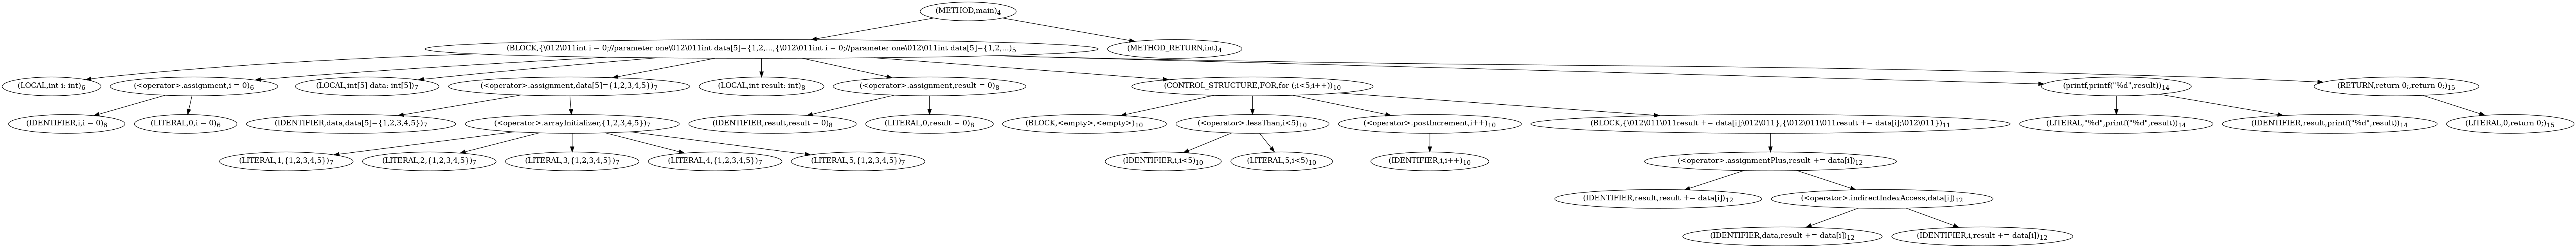
\includegraphics[width=0.3\textwidth]{figures/ast1}  
      \label{fig:ast1} %引用标签
  }
  \subfigure[代码片段2对应的AST]{ %第二张子图
      \centering    %子图居中
      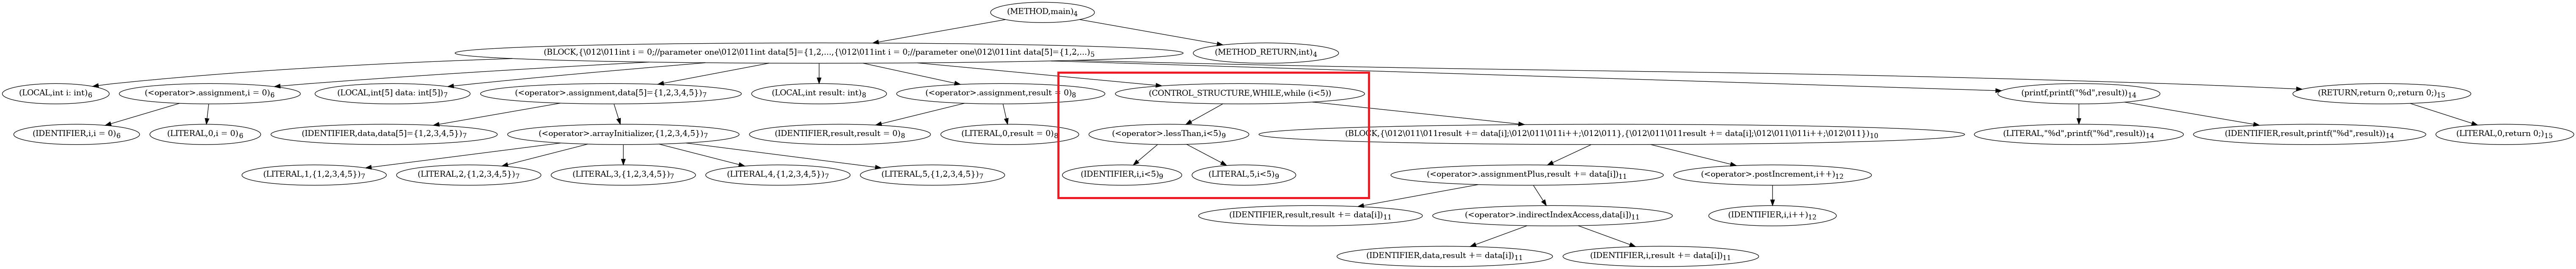
\includegraphics[width=0.3\textwidth]{figures/ast2}
      \label{fig:ast2} %引用标签
  }
  \subfigure[代码片段3对应的AST]{ %第三张子图
      \centering    %子图居中
      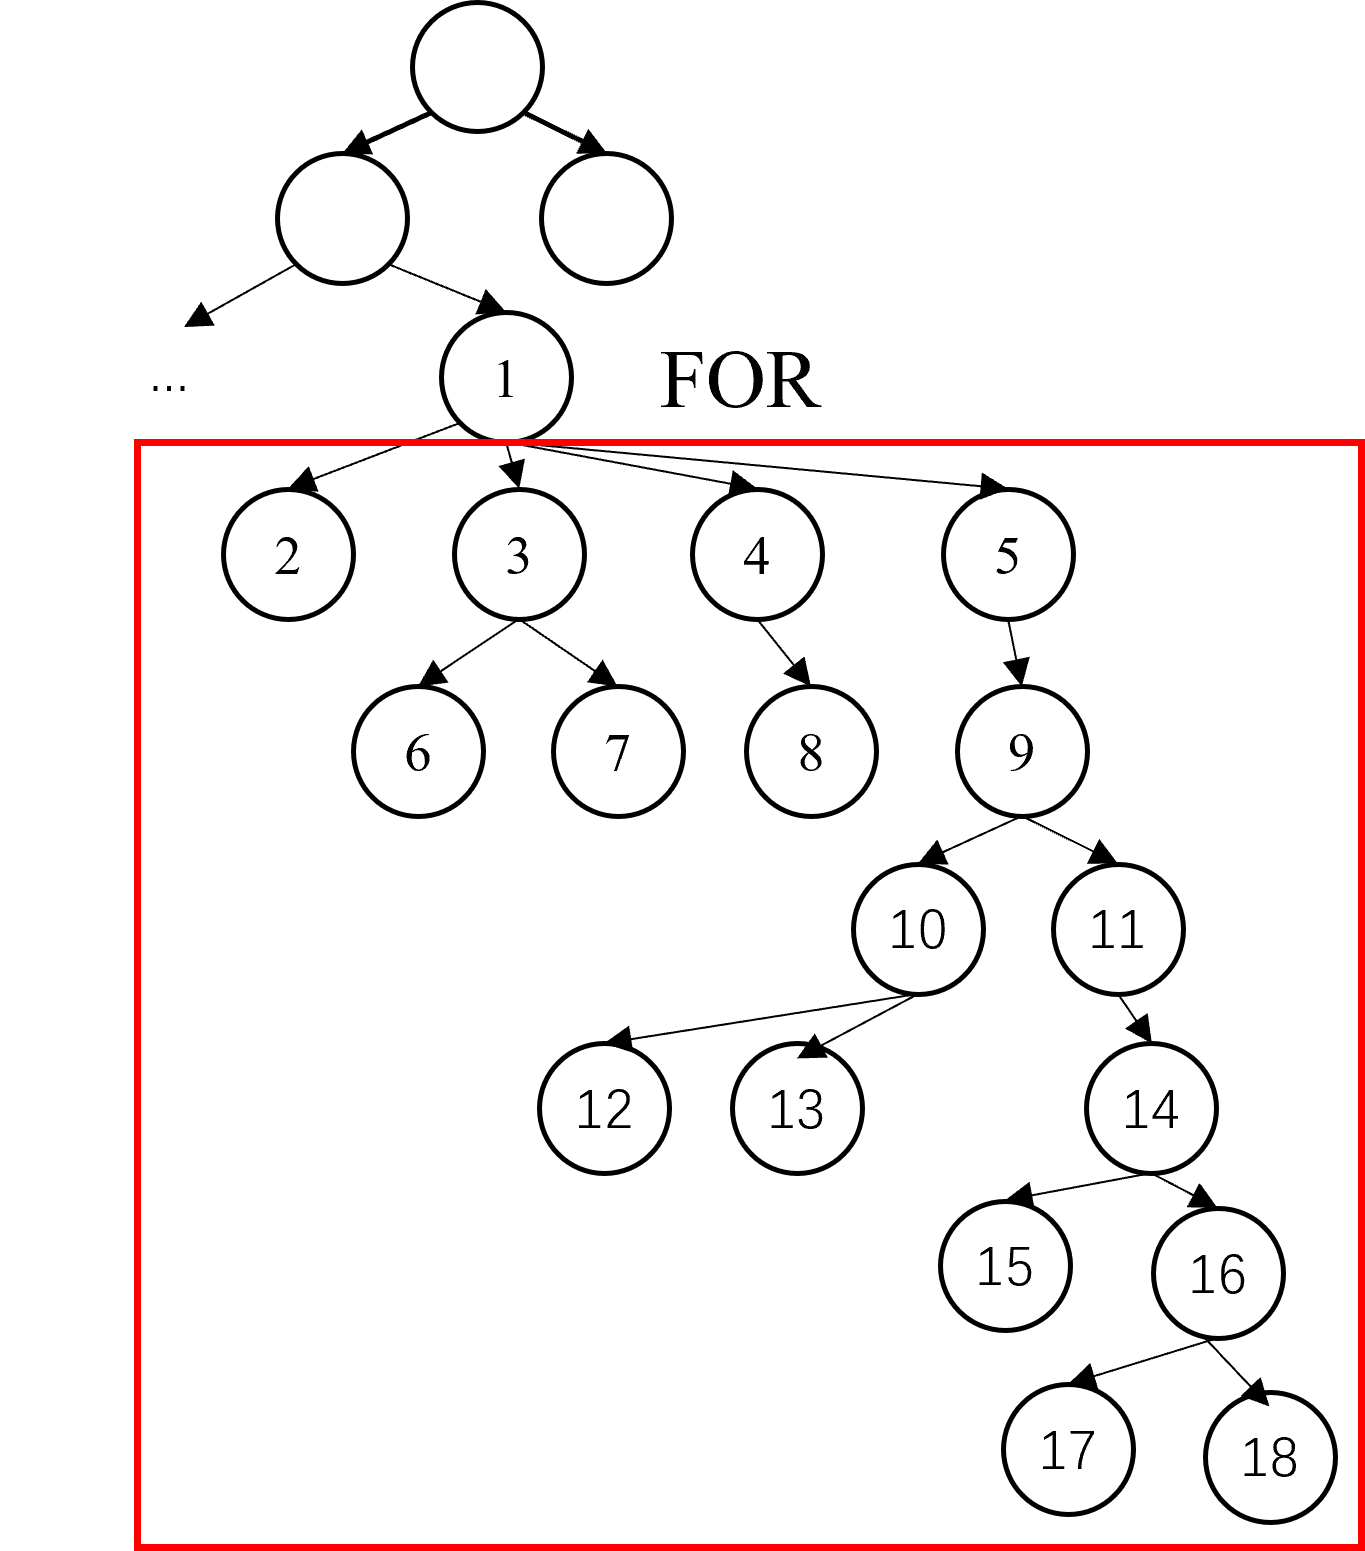
\includegraphics[width=0.25\textwidth]{figures/ast3}
      \label{fig:ast3} %引用标签
  }
  \caption{示例源代码对应的抽象语法树}    %大图名称
  \label{fig:astcode}    %图片引用标记
\end{figure}

接下来,本章提出的基于子树划分的抽象语法树表征学习方法的实现如图\ref{fig:ast}所示。该方法的输入是一对代码片段$C_{a},C_{b}$对应的抽象语法树,表示为$AST_{a},AST_{b}$,输出是$C_{a},C_{b}$对应的结构特征向量 $V_{a}^{AST},V_{b}^{AST}$,整体采用Siamese架构,两个子网络共享权值,从下到上,主要包括子树划分、子树表征、树表征三个阶段。

\begin{figure}[H]
  \centering
  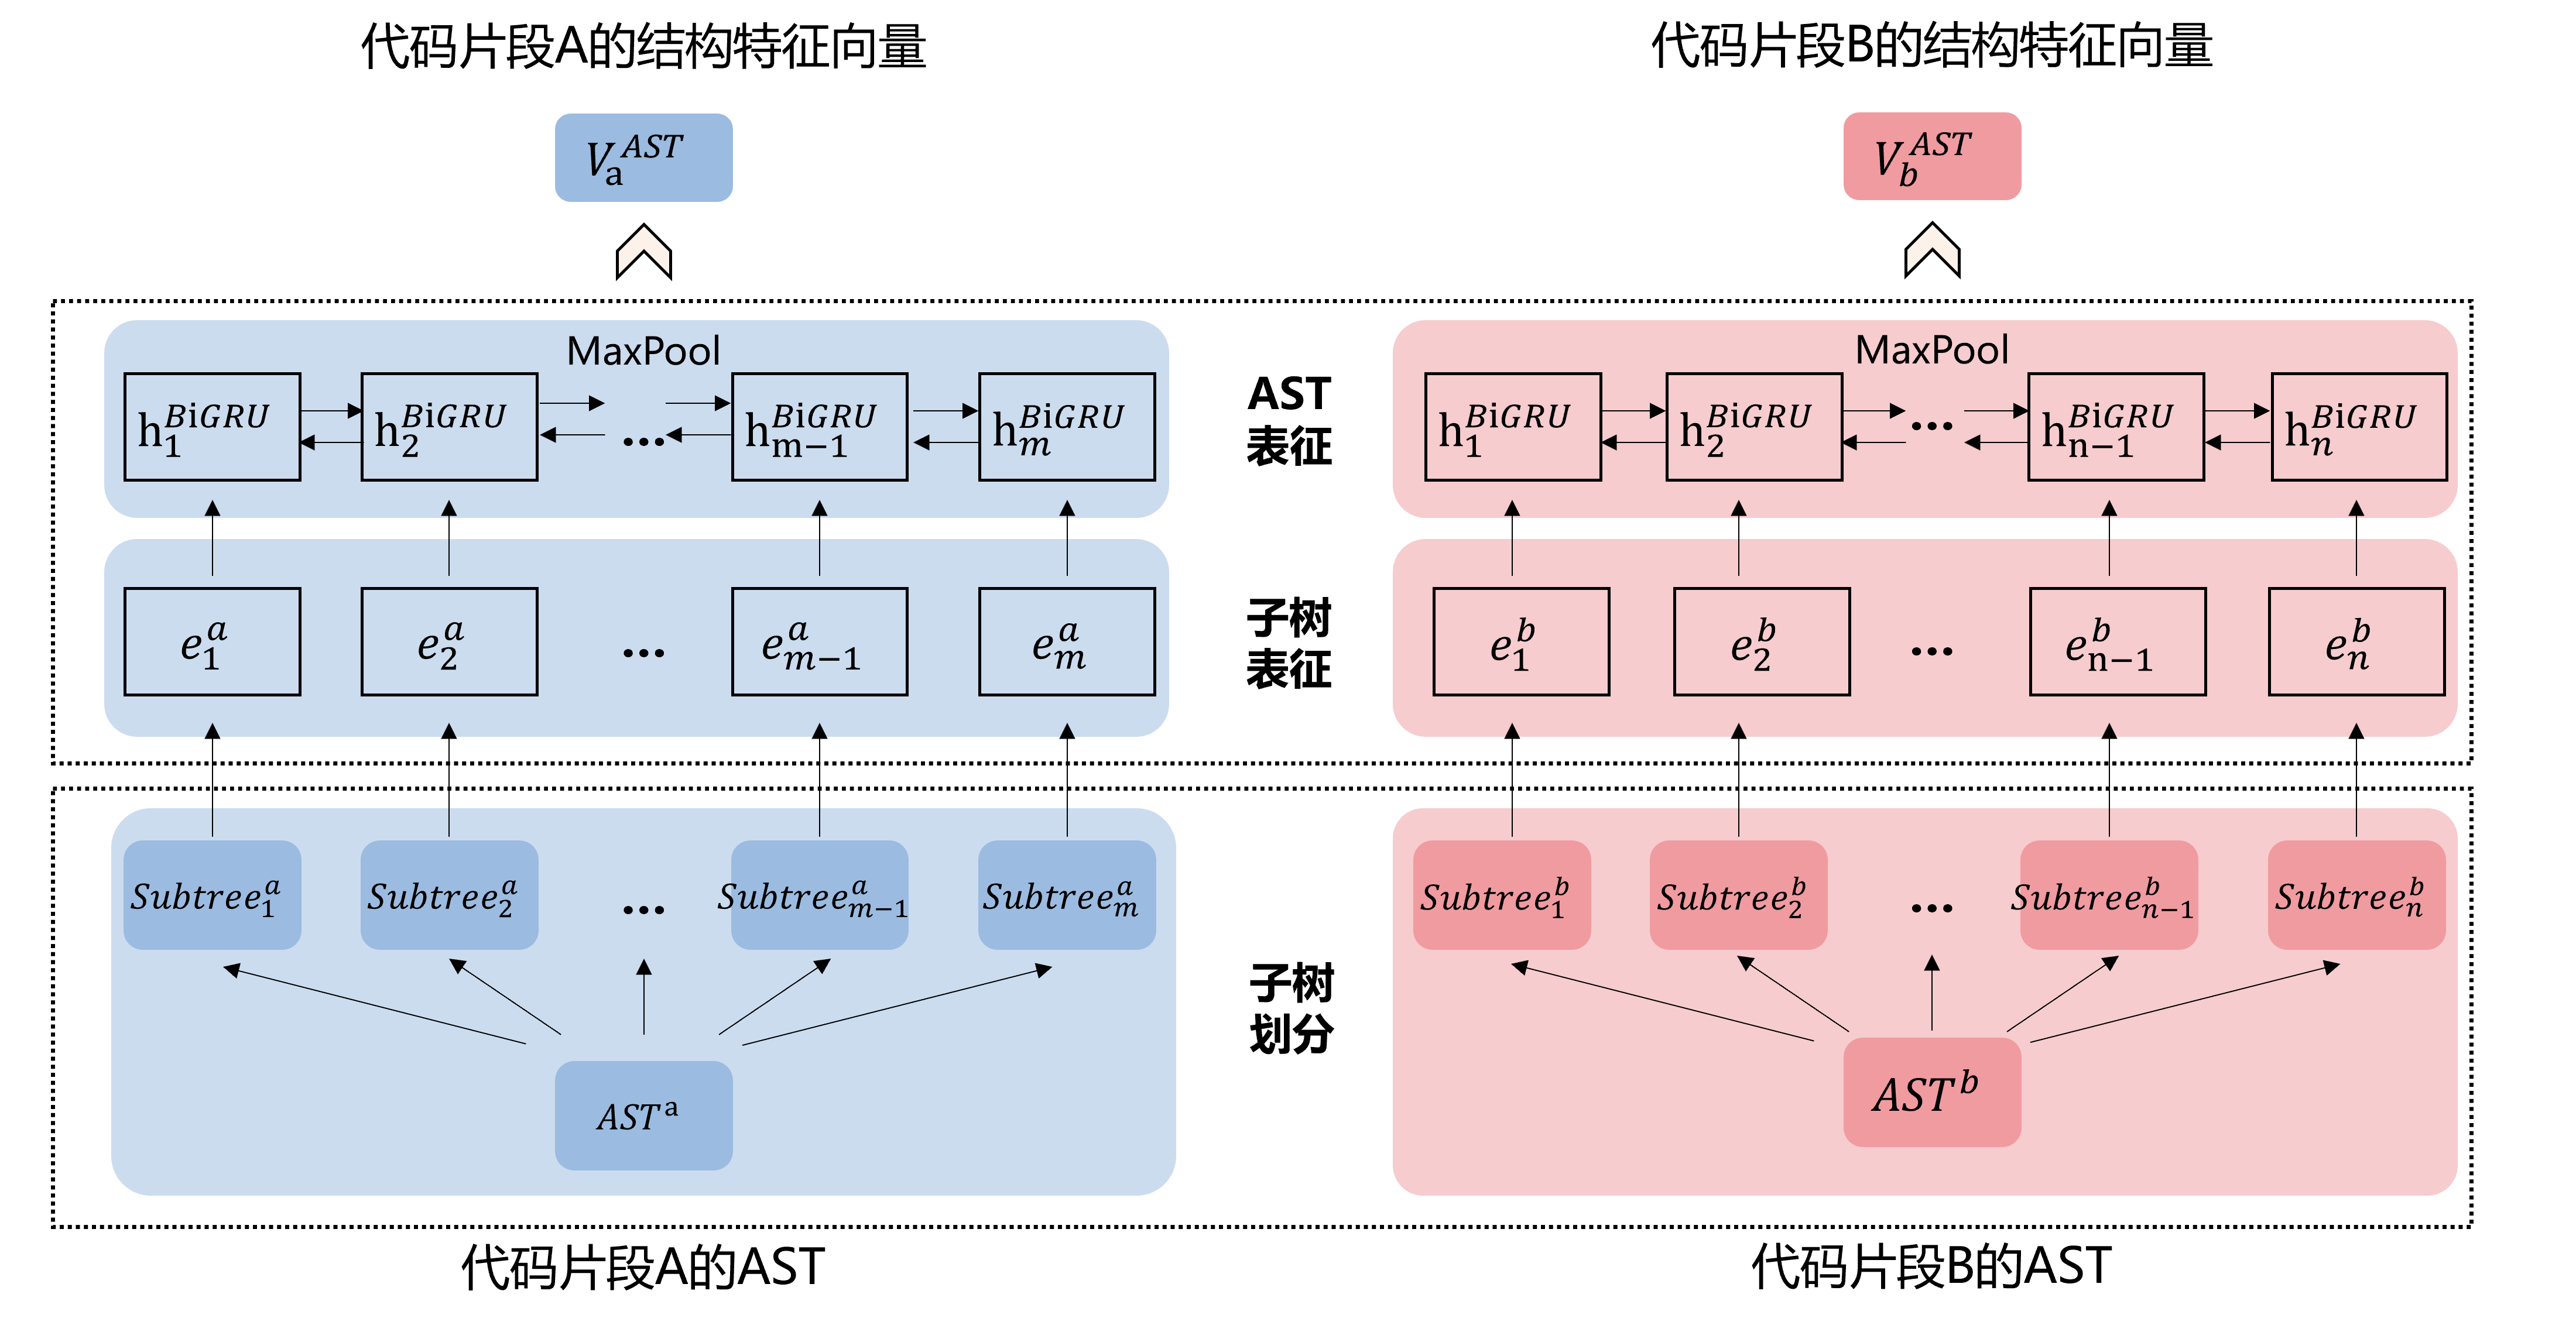
\includegraphics[width=0.9\textwidth]{figures/ast}
  \caption{基于子树划分的抽象语法树表征学习方法实现}\label{fig:ast}
\end{figure}

具体来说,在子树划分阶段,对于代码片段$C_{a}$,经过代码分析工具Joern生成得到抽象语法树$AST_{a}$,通过子树划分算法,可以得到子树序列,用$\left(SubTree_{1}^{a},SubTree_{2}^{a},\ldots,\notag \right.\\\left.SubTree_{1}^{m}\right)$表示,$m$是子树序列的长度。其子树划分过程可以表示为公式\ref{e4.8}:

\begin{equation}\label{e4.8}
  \begin{split}
    \left(SubTree_{1}^{a},SubTree_{2}^{a},\ldots,SubTree_{m}^{a}\right) = split\_AST \left(AST_{a}\right)
  \end{split}
\end{equation}

经过子树划分后,代码片段$C_{a}$生成了子树序列$\left(SubTree_{1}^{a},SubTree_{2}^{a},\ldots,SubTree_{m}^{a}\right)$。使用同样的划分方法,可以得到代码片段$C_{b}$生成了子树序列$\left(SubTree_{1}^{b},SubTree_{2}^{b},\ldots,\notag \right.\\\left.SubTree_{n}^{b}\right)$,$n$是代码片段$C_b$对应的子树序列长度。

在树表征阶段,首先将代码片段的子树序列作为输入,使用基于树的卷积神经网络模型进行编码,得到每个子树对应的语句向量$\left( e_{1}^{a},e_{2}^{a},\ldots,e_{m}^{a}\right)$。然后,使用双向门控循环单元(BiGRU)来模拟语句的自然性,通过最大池化层将BiGRU的隐藏状态采样到单个固定长度的向量$V_{a}^{AST}$中,作为最终的抽象语法树表示,即结构特征向量。具体的处理过程如公式\ref{e4.9}
\begin{equation}\label{e4.9}
  \begin{split}
    h_{1}^{aBiGRU},h_{2}^{aBiGRU},\ldots,h_{n}^{aBiGRU} = BiGRU \left(e_{1}^{a},e_{2}^{a},\ldots,e_{m}^{a}\right) \\
    V_{a}^{AST} = MaxPool \left( h_{1}^{aBiGRU},h_{2}^{aBiGRU},\ldots,h_{n}^{aBiGRU} \right)
  \end{split}
\end{equation}

同样,可以使用相同的计算以子树序列$\left(SubTree_{1}^{b},SubTree_{2}^{b},\ldots,SubTree_{n}^{b}\right)$作为输入为代码片段$C_{b}$计算$V_{b}^{AST}$。


\section{实验验证}
\label{sec:ASTExperiment}
为了验证基于子树划分的抽象语法树表征学习方法的有效性,本节开展实验验证。首先,介绍了实验的具体设计,接着对子树划分、树表征模型进行消融实验。

\subsection{实验设计}
\label{subsec:ASTDesign}

本节使用与\ref{sec:TokenExperiment}节中同样的实验环境、数据集对基于子树划分的抽象语法树表征学习方法进行对比实验。本实验使用代码分析工具Joern获取数据集中代码片段的抽象语法树AST,然后使用基于树的卷积神经网络训练子树嵌入,并将嵌入向量大小设置为128。同样选取常用的精确率(Precision)、召回率(Recall)、F1值作为评估指标。

\subsection{实验结果}
\label{subsec:TokenResult}

(1)拆分AST粒度的实验结果

为了探究子树拆分对抽象语法树表征实验结果的影响,本文设计了三种不同的方法来处理AST。首先,将代码片段原始的完整抽象语法树视为一个特殊的子树,不进行拆分,用AST-Full表示,即粒度威威整棵树,完全不进行子树划分。其次,将AST的所有节点均提取为子树,用AST-Node表示,即粒度精确到每个节点。最后,根据子树划分块来处理抽象语法树,用AST-Block表示。本实验采取单一变量原则,仅修改AST拆分粒度,后续子树的编码采用相同的基于树的卷积神经网络,采用双向GRU处理整棵树的嵌入。具体实验结果如表\ref{tab:subtree}所示。


\begin{table}[htp] 
  \centering
  \caption{抽象语法树子树划分对实验结果的影响} 
  \label{tab:subtree}
  %\renewcommand{\arraystretch}{1.1}
  \begin{tabular*}{0.9\textwidth}{@{\extracolsep{\fill}}cccc}
  \toprule
  \multirow{2}{*}{AST划分粒度} & \multicolumn{3}{c}{POJ104} \\
  \cmidrule{2-4} 
   & 准确率P(\%) & 召回率R(\%) & F1值(\%)  \\  
  \midrule
    AST-Full			&85.74	  &87.72		   &86.70 \\
    AST-Node      &89.78	  &87.88		   &88.82 \\
    AST-Block			&92.75	  &87.62		   &90.11 \\
  \bottomrule
  \end{tabular*}
\end{table}

从表\ref{tab:subtree}可以看出,AST-Block优于AST-Full和AST-Node。探究其原因,AST-Full未进行子树划分,因此抽象语法树通常规模过大,在模型训练过程中容易造成梯度消失,权重无法及时更新,同时无法提取子树粒度的代码信息,从而导致代码检测的效果最差。而AST-Node将树的每一个节点都设为子树,导致基于树卷积的神经网络输入规模过大,影响检测效率。AST-Block很好地平衡了子树大小和句法信息的丰富性,其F1值达到了90.11。因此,得出以下结论:本章提出的子树划分算法对代码克隆的检测具有一定的优势。

(2)树表征模型实验结果

为了探究树表征模型GRU对实验结果的影响,本文在子树划分的基础上,将GRU模型与LSTM模型进行对比,结果如表\ref{tab:tree2}所示。

其中,GRU、LSTM均基于Pytorch1.10实现,其参数设置为:\ding{172} 子树划分:采用AST-Block的划分方法。\ding{173} 子树的表征均采用基于树的卷积神经网络,整树的表征模型的隐藏层维度设置为128,模型使用二元交叉熵作为损失函数,使用Adam优化器来训练模型参数,其中,学习率Learning\_rate设置为0.001,Dropout为0.5,训练批次Epochs为50,批处理大小Batch\_size为32,阈值Threshold为0.5,当相似度超过0.5,输入的代码对被判定为真克隆对,否则被判定为假克隆对。参数的确定是通过多次调试后选择最优参数作为最后的结果。

\begin{table}[htp]  
  \centering  
  \caption{树表征模型对实验结果的影响}   
  \label{tab:tree2}
  %\renewcommand{\arraystretch}{1.1}  
  \begin{tabular*}{0.9\textwidth}{@{\extracolsep{\fill}}cccc}  
  \toprule  
  表征模型 & 准确率P(\%) & 召回率R(\%) & F1值(\%)  \\  
  \midrule
  LSTM			  & 92.21	  & 83.52	 & 87.65		\\  
  GRU		      & 92.75	  & 87.62	 & 90.11 \\ 
  \bottomrule  
  \end{tabular*}  
\end{table}

基于对表\ref{tab:tree2}数据的分析,可以得到以下结论:(1)在对整树进行表征的过程中,LSTM模型的整体表现略差于GRU,准确率整体相当,两者均可以解决传统循环神经网络中存在的梯度消失问题。(2)LSTM模型的召回率比GRU低4.10\%。深究其原因,可能是因为LSTM由于单元内包含三个门,计算机制复杂,所以影响其召回率,而GRU模型结构相对简单,只有两个门,参数数量较少,模型收敛速度更快,计算效率更高。因此,在树维度的代码表征模型选取上,本文更倾向于GRU。


(3)树表征可视化

为了更直观地展示本文提出的基于子树划分的抽象语法树表征学习方法的有效性,本实验同样使用t-SNE技术将高维结构特征向量可视化,按照预先设定的参数,树表征学习后生成的张量维度是128,采用t-SNE技术将128维的张量转换为2维,得到的样本表征结果如图\ref{fig:origintwo}所示。

\begin{figure}[H] 
  \centering  %居中
  \subfigure[初始向量可视化]{   %第一张子图
      \centering    %子图居中
      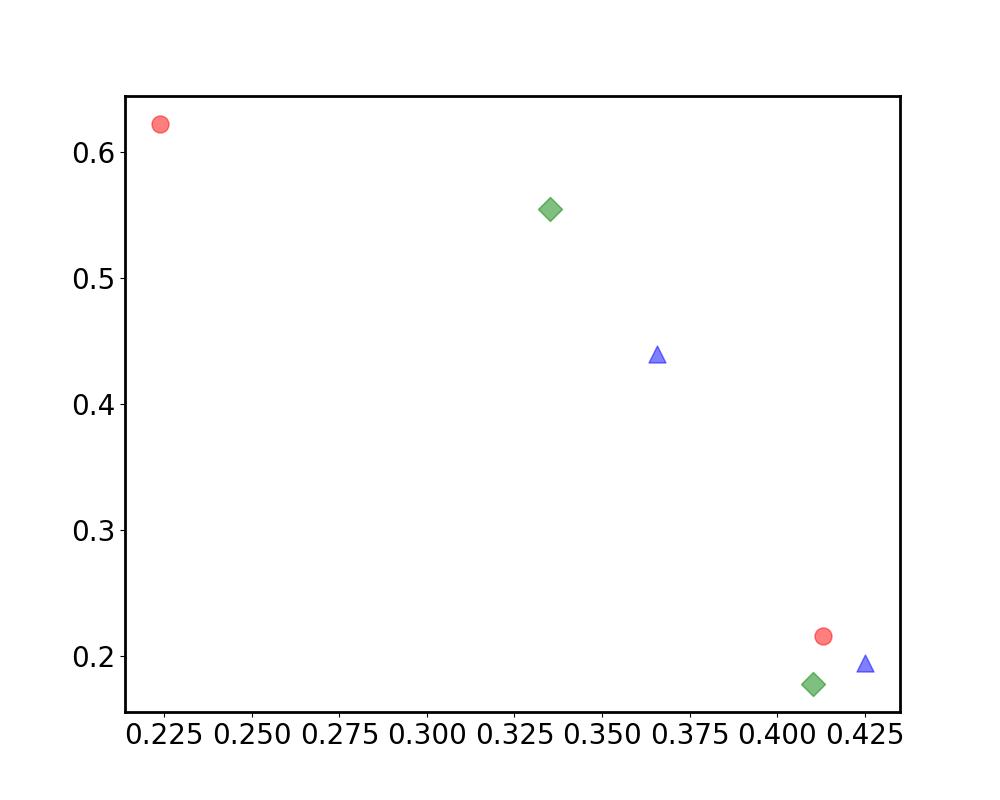
\includegraphics[width=0.45\textwidth]{figures/origin.png} 
      \label{fig:origint} %引用标签
  }
  \subfigure[结构特征向量可视化]{ %第二张子图
      \centering    %子图居中
      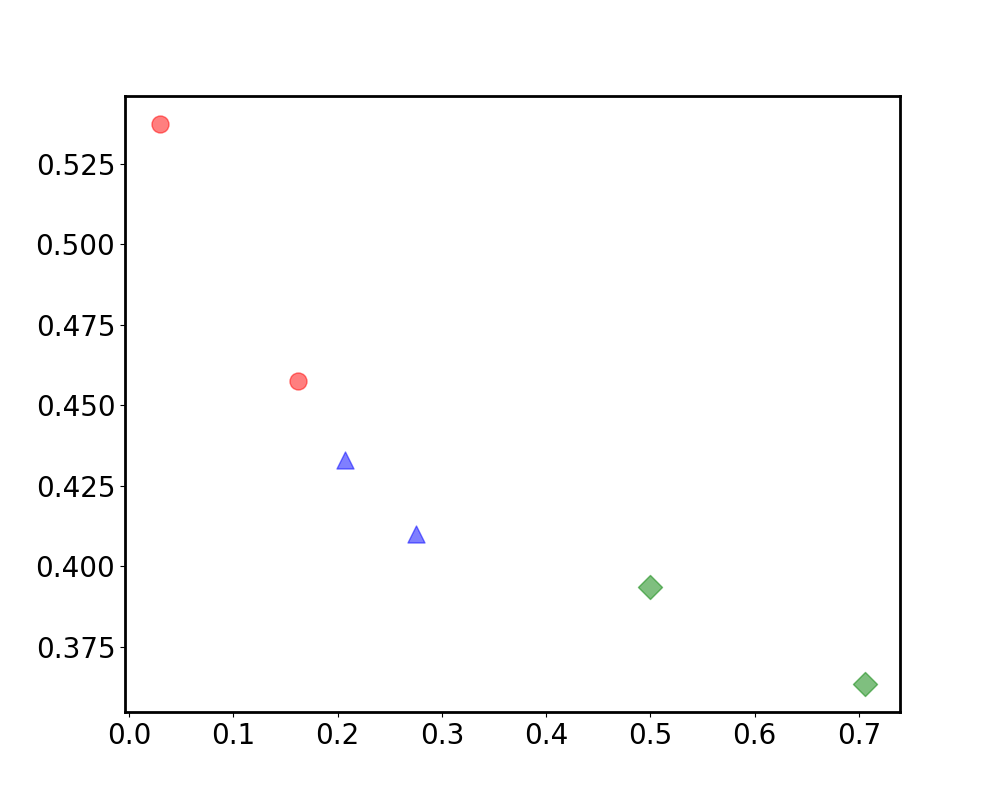
\includegraphics[width=0.45\textwidth]{figures/origin2.png}
      \label{fig:origin2} %引用标签
  }
  \caption{t-SNE技术降维后的结构特征向量可视化结果}    %大图名称
  \label{fig:origintwo}    %图片引用标记
\end{figure}

如图\ref{fig:origintwo}所示,\ref{fig:origint}和\ref{subsec:TokenResult}可视化实验中采用的代码片段相同,而\ref{fig:origin2}中,向量空间的所有点是代码片段通过树表征学习后得到的结构特征向量可视化结果。可以看到互为真克隆对的代码片段在经过树表征模型训练后相互聚。并且,与Token维度表征后的属性特征向量可视化结果\ref{fig:origin1}相比,树维度的可视化结果更优秀,说明树维度相比于Token维度包含了更多代码信息,模型有效地学习到了更有效的代码表征。


\section{本章小结}
\label{sec:Summary4}
本章主要对RLCCD中基于子树划分的抽象语法树表征学习方法的设计与实现进行详细阐述。首先介绍了抽象语法树维度的研究动机,其次介绍了抽象语法树表征学习的方法设计,具体论述了其整体框架、子树划分、树表征学习,接着开展实验验证,结果表明了此方法的有效性和模型的准确性。



